\documentclass[notes, c, 11pt, xcolor=dvipsnames, hyperref={colorlinks,citecolor=Maroon,linkcolor=Maroon,urlcolor=RoyalBlue}]{beamer}

% print notes only:
%\documentclass[notes=only, c, 11pt, xcolor=dvipsnames, hyperref={colorlinks,citecolor=Maroon,linkcolor=Maroon,urlcolor=RoyalBlue}]{beamer}

%print only frames:
%\documentclass[c, 11pt, xcolor=dvipsnames, hyperref={colorlinks,citecolor=Maroon,linkcolor=Maroon,urlcolor=RoyalBlue}]{beamer}

% print handouts:
%\documentclass[handout, c, 11pt, xcolor=svgnames, hyperref={colorlinks,citecolor=DeepPink4,linkcolor=DarkRed,urlcolor=DarkBlue}]{beamer} 
%\usepackage{pgfpages}
%\pgfpagesuselayout{4 on 1}[a4paper, border shrink=5mm, landscape]

\setbeamerfont{note page}{size=\tiny}

\usepackage[english]{babel}
\usepackage[latin1]{inputenc}
\usepackage[T1]{fontenc}

\mode<presentation> {
	
	% The Beamer class comes with a number of default slide themes
	% which change the colors and layouts of slides. Below this is a list
	% of all the themes, uncomment each in turn to see what they look like.
	
	%\usetheme{default}
	%\usetheme{AnnArbor}
	%\usetheme{Antibes}
	%\usetheme{Bergen}
	%\usetheme{Berkeley}
	%\usetheme{Berlin}
	%\usetheme{Boadilla}
	\usetheme{CambridgeUS}
	%\usetheme{Copenhagen}
	%\usetheme{Darmstadt}
	%\usetheme{Dresden}
	%\usetheme{Frankfurt}
	%\usetheme{Goettingen}
	%\usetheme{Hannover}
	%\usetheme{Ilmenau}
	%\usetheme{JuanLesPins}
	%\usetheme{Luebeck}
	%\usetheme{Madrid}
	%\usetheme{Malmoe}
	%\usetheme{Marburg}
	%\usetheme{Montpellier}
	%\usetheme{PaloAlto}
	%\usetheme{Pittsburgh}
	%\usetheme{Rochester}
	%\usetheme{Singapore}
	%\usetheme{Szeged}
	%\usetheme{Warsaw}
	
	% As well as themes, the Beamer class has a number of color themes
	% for any slide theme. Uncomment each of these in turn to see how it
	% changes the colors of your current slide theme.
	
	%\usecolortheme{albatross}
	%\usecolortheme{beaver}
	%\usecolortheme{beetle}
	%\usecolortheme{crane}
	%\usecolortheme{dolphin}
	%\usecolortheme{dove}
	%\usecolortheme{fly}
	%\usecolortheme{lily}
	%\usecolortheme{orchid}
	%\usecolortheme{rose}
	%\usecolortheme{seagull}
	%\usecolortheme{seahorse}
	%\usecolortheme{whale}
	%\usecolortheme{wolverine}
	
	\usefonttheme{professionalfonts}
	
	\usepackage{times}
	\usepackage{tikz}
	\usetikzlibrary{arrows,shapes}
	
	%\setbeamertemplate{footline} % To remove the footer line in all slides uncomment this line
	%\setbeamertemplate{footline}[page number] % To replace the footer line in all slides with a simple slide count uncomment this line
	\setbeamertemplate{headline} % to remove header with navigation tree
	
	\setbeamertemplate{navigation symbols}{} % To remove the navigation symbols from the bottom of all slides uncomment this line
}

\usepackage{amsmath,mathtools}
\usetikzlibrary{matrix, fit, backgrounds}

\usepackage{graphicx} % Allows including images
\usepackage{booktabs} % Allows the use of \toprule, \midrule and \bottomrule in tables
\usepackage{subcaption}
\usepackage{tabularx}

\usepackage{fancyvrb}

\usetikzlibrary{mindmap,trees,shadows,backgrounds}

%\tikzset{every node/.append style={scale=0.6}}    

\usepackage{array,multirow}
\usepackage{changepage}

\usepackage[backend=biber, style=authoryear-comp, citestyle=authoryear-comp, firstinits=true, url=false, doi=false, eprint=false, dashed=false, maxbibnames=99]{biblatex}
\addbibresource{bib.bib}

%----------------------------------------------------------------------------------------
%	TITLE PAGE
%----------------------------------------------------------------------------------------

\title[Webinar for ISDS R Group]{Building meaningful machine learning models for disease prediction} % The short title appears at the bottom of every slide, the full title is only on the title page

\author{Dr Shirin Glander} % Your name
\institute[] % Your institution as it will appear on the bottom of every slide, may be shorthand to save space
{
	Dep. of Genetic Epidemiology \\
	Institute of Human Genetics \\
	University of M\"unster
	
	\vspace{0.5cm} 
	
	\href{mailto:shirin.glander@wwu.de}{shirin.glander@wwu.de} \\
	
	\vspace{0.5cm} 
	
	\href{https://shiring.github.io}{https://shiring.github.io} \\
	
	\href{https://github.com/ShirinG}{https://github.com/ShirinG}
	
}
\date{Friday, 31\textsuperscript{st} March 2017} 

\AtBeginSection[]{
	\begin{frame}
		\vfill
		\centering
		\begin{beamercolorbox}[sep=8pt,center,shadow=true,rounded=true]{title}
			\usebeamerfont{title}\insertsectionhead\par%
		\end{beamercolorbox}
		\vfill
	\end{frame}
}

%\renewcommand{\thefootnote}{$\star$} 

%%%%%%%%%%%%%%%%%%%%%
%	TITLE PAGE
%%%%%%%%%%%%%%%%%%%%%

\begin{document}
	
	\begin{frame}
		\titlepage
	\end{frame}
	
\note{
	\begin{itemize}
		\item Welcome everybody!
		\item Thank you very much for the invitation and the opportunity to present this talk
		\item I will go over my work on using machine learning models in disease prediction
		\item I want to specifically give a hands-on demonstration of how you can build meaningful models yourselves using R
		\item I will demonstrate how to evaluate model performance and
		\item how to optimize models to address different disease-related questions
	\end{itemize}
}

%%%%%%%%%%%%%%%%%%%%%
%	ABOUT ME
%%%%%%%%%%%%%%%%%%%%%

\begin{frame}
	\frametitle{About me}
	
	\begin{columns}
		\column{0.15\textwidth}	
	
		\column{0.8\textwidth}	
	\begin{itemize}		
		\item[since 2015] Bioinformatics Postdoc \\
							Next Generation Sequencing \\
							autoinflammatory diseases \& \\
							innate immunity \\[5mm]
		\item[2011 - 2015] PhD in Biology \\
							Is the immune system of plants required to adapt to flowering time change? \\[5mm]
		\item[2005 - 2011] BSc and MSc of Science in Biology \\
							evolutionary genetics, \\ immune memory in Drosophila \\				
	\end{itemize}

	\column{0.05\textwidth}	
	
	\begin{tikzpicture}[remember picture,overlay]
	\node[xshift=-2.1cm,yshift=-2.5cm] at (current page.north east) {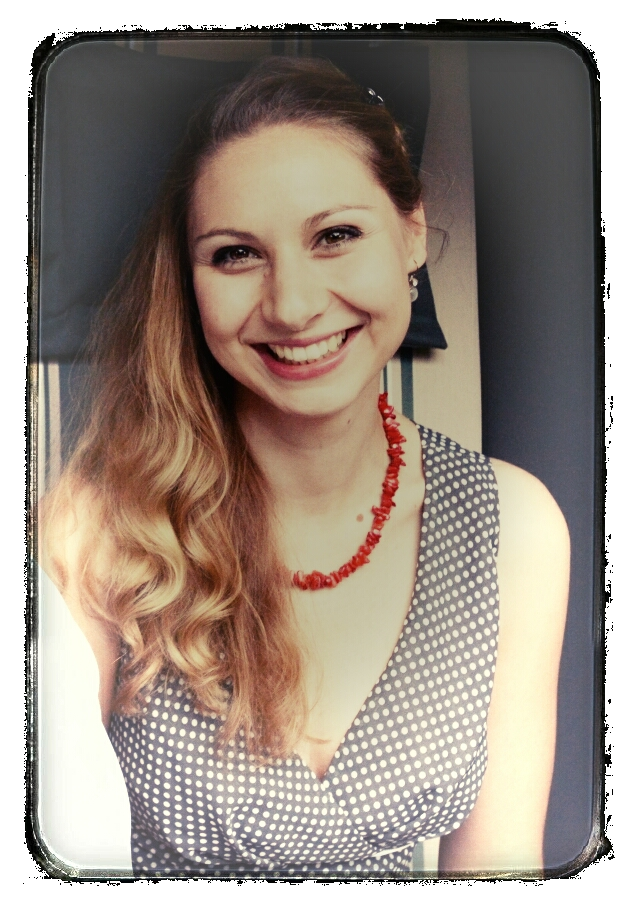
\includegraphics[width=3cm]{images/bild.png}};
	\end{tikzpicture}

	\end{columns}
\end{frame}

\note{
	\begin{itemize}
		\item Before I start, I want to quickly introduce myself:
		\item I am a bioinformatics postdoc
		\item working with next generation sequencing data,
		\item like RNA-seq for transcriptomics,
		\item whole genome sequencing for variant analysis,
		\item ATAC- or Chip-seq for chromatin and epigenetic information.
		\item My own research focuses on questions relating to autoinflammatory diseases
		\item and innate immune mechanisms
	\end{itemize}
	
	\begin{itemize}
		\item I earned my PhD in biology from the University of M�nster in 2015
		\item working with RNA-seq data to determine how plant defense has co-evolved with and potentially shaped different life-history strategies
	\end{itemize}
	
	\begin{itemize}
		\item Before that, during my BSc and MSc I worked on questions about evolutionary genetics and immune memory in Drosophila
		\end{itemize}
}

%%%%%%%%%%%%%%%%%%%%%
%	TABLE OF CONTENTS
%%%%%%%%%%%%%%%%%%%%%

	\begin{frame}[c]
		\frametitle{Table of contents}
		\alert{Building meaningful machine learning models for disease prediction}
		\vspace{0.5cm}
			\tableofcontents[hideallsubsections]

	\end{frame}

\note{
	\begin{itemize}
		\item Now, let's start with the topic about which you're here:
		\item Machine learning is a powerful approach for developing sophisticated, \\
			automatic, and objective models for the analysis of complex biomedical data
		\item Machine learning promises to help physicians make near-perfect diagnoses, ...
		\item ... choose the best medications for their patients, ...
		\item ... predict readmissions, ...
		\item ... identify patients at high-risk for poor outcomes, ...
		\item ... and in general improve patients' health while minimizing costs. 
	\end{itemize}
	
	\begin{itemize}
		\item I titled my talk: "Building meaningful machine learning models for disease prediction"
		\item with the emphasis on \textbf{meaningful}
		\item So, first, I want to introduce to you what it is I mean exactly with \textbf{meaningful models}
		\item Then, I will give you a few examples of how machine learning is currently being used in disease modeling and clinical data science
		\item Before I delve into the nitty-gritty of modeling, I will quickly recap the most important concepts of ML
		\item And finally, I will show how to build ML models in R
		\item and how to evaluate the performance of such models
	\end{itemize}
}

%%%%%%%%%%%%%%%%%%%%%
%	SECTION
%	What makes a model meaningful?
%%%%%%%%%%%%%%%%%%%%%

\section{What makes a model meaningful?}

\begin{frame}
	\frametitle{What makes a model meaningful?}
	
	\begin{itemize}
		\item creating ML models is relatively easy
		\item creating \alert{good or meaningful} models is hard
	\end{itemize}
	
	\vspace{0.2cm}
	\alert{\textsl{Meaningful} models}
	\vspace{0.2cm}
	
	\begin{itemize}
		\item are generalizable
		\item answer the question(s) posed...
		\item ... with sufficient accuracy to be trustworthy
	\end{itemize}

	\vspace{0.2cm}

	\begin{center}
		{\Large \alert{Accuracy depends on the problem!}}
		
		\vspace{0.5cm}
		
		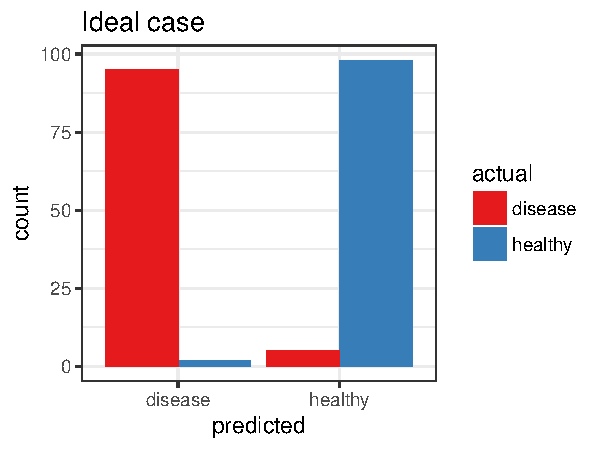
\includegraphics[width=0.33\textwidth]{images/meaningful_1}
		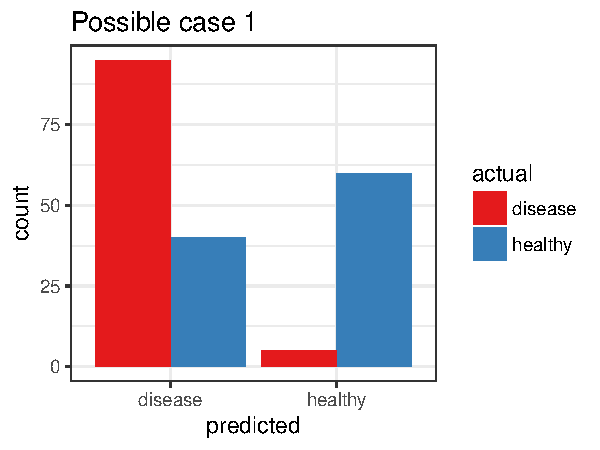
\includegraphics[width=0.33\textwidth]{images/meaningful_2}
		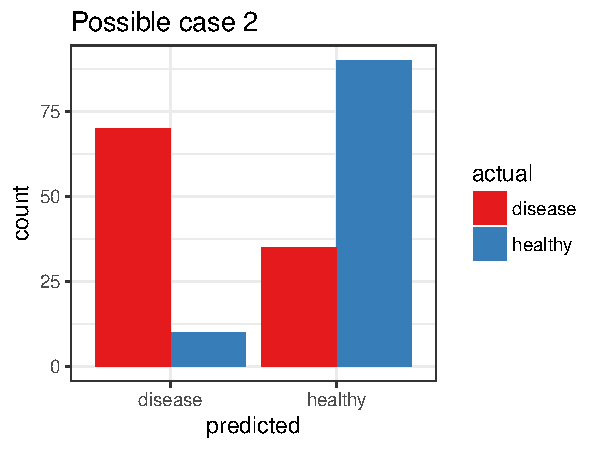
\includegraphics[width=0.33\textwidth]{images/meaningful_3}
	\end{center}
	
\end{frame}

\note{
	\begin{itemize}
		\item With a little bit of practice, anybody can build machine learning models
		\item what is hard though, is to build 'good' or 'meaningful' models
		\item I want to begin with an introduction to the main question of my talk: 
		\item what makes a model \textsl{good} or \textsl{meaningful}?
	\end{itemize}
	
	\begin{enumerate}
		\item it needs to be generalizable, i.e. it needs to perform well on unseen data
		\item It answers a \textbf{specific} question or addresses a specific problem, \\
			e.g. does a mammogram image show a healthy breast or is there a tumor? \\
			Or does an ECG show a normal heart rhythm or arrhythmia?
		\item And it produces a correct outcome (e.g. a diagnosis) often enough that we trust it!
	\end{enumerate}
	
	\begin{itemize}
		\item If we build models, we therefore need to evaluate its accuracy 
		\item before we can decide whether it is trustworthy enough to implement in real-life, 
		\item like in a hospital where it could e.g. assist doctors in making decisions on treatment
	\end{itemize}

	\begin{itemize}
		\item But what exactly is \textsl{high accuracy} can not be defined with a one-size-fits-all approach: 
		\item it depends on the problem we want to model. 	
		\item a model needs to perform well in the real world, not in the lab (i.e. on training data)
		\item just because a model performs well in the lab, doesn't mean it will also perform well in deployment
		\item the context might change: distribution, missing data, noise, class size, etc.
	\end{itemize}
}

\note{
	Let me illustrate what I mean with the following examples:
	\begin{itemize}
		\item \alert{Ideal case:} Of course, we all want to achieve ideal modeling results where overall prediction accuracy is very high. \\ 
		With a model like that, we can be very confident that a healthy person is indeed healthy and a sick person is not. \\
		\item But in reality, we often achieve prediction accuracies that are much less nice. \\
		\item \alert{Scenarios 1 and 2:} Le's consider two possible scenarios: 
		\item in scenario 1, we can be very confident that a person who got classified as "healthy" is indeed healthy, \\ 
		while a person who has been diagnosed as diseased might as well be healthy based on these prediction accuracies
		\item in case 2, it is the other way around.
		\item We now need to make a decision which scenario is better and in which direction we want to optimize our model: \\ 
		do we rather want to refer a few healthy people for further checking because the model predicted them as diseased? \\ 
		Or do we rather want to be as certain as possible that a predicted disease is actually true \\ 
		and accept that we might miss a few disease cases?
	\end{itemize}
}

%%%%%%%%%%%%%%%%%%%%%
%	SECTION
%	Machine Learning (ML) in disease modeling
%%%%%%%%%%%%%%%%%%%%%

\section{Machine Learning (ML) in disease modeling}

\begin{frame}
	\frametitle{ML in disease modeling}
	
	\begin{itemize}
		\item tools that can interpret "big medical data" 
		\item and provide fast, accurate and actionable information
		\item for precision or personalized medicine
	\end{itemize}

	\vspace{0.5cm}

	\alert{Examples:} 
	\begin{itemize}
		\item computer-aided diagnosis of breast cancer \\ from mammograms\footcite{Kunio}
		\item identifying gene defects with facial recognition \\ software\footcite{Levenson}
		\item identifying signatures of Brain Cancer \\ from MRSI \footcite{doi:10.1146/annurev.bioeng.8.061505.095802}
		\item ... and many more ...
	\end{itemize}

	\begin{tikzpicture}[remember picture,overlay]
	\node[xshift=-2cm,yshift=4cm] at (current page.south east) {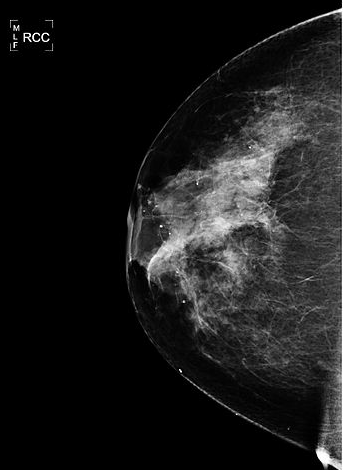
\includegraphics[width=3cm]{images/mammogram}};
	\node[xshift=-3cm,yshift=0.8cm] at (current page.south east) {\footnotesize{\textit{Image source: Wikimedia Commons}}};
	\end{tikzpicture}

	%\footfullcite{}
	
\end{frame}

\note{
	\begin{itemize}
		\item there is not a place in medicine where AI doesn't have potential applications:
		\item more data is being collected that needs to be interpretated
		\item increasingly data driven diagnosis, e.g. in radiology
		\item image recognition of e.g. tumors or pneumonia in medical images
		\item similar to training ML models to recognize images of cats (classification in images)
		\item ML allows incorporation of data from heterogenous inputs: 
		\item clinical, genomics, drugs, electronic health records, etc.
		\item = personalised medicine
	\end{itemize}

	\begin{itemize}
		\item A key aspect of precision medicine is the development of informatics tools 
		\item that can analyze and interpret 'big data' sets 
		\item in an automated and adaptive fashion 
		\item while providing accurate and actionable clinical information
		\item ML based models can improve detection, diagnosis, and therapeutic monitoring of disease
	\end{itemize}

	\begin{itemize}
		\item you can find things with ML that you wouldn't be able to find otherwise
		\item many models today perform better than humans!
		\item a patient with a rare difficult condition can be matched to similar cases from the past
		\item faster diagnosis, better treatment
	\end{itemize}
}

\note{	
	\begin{itemize}
		\item identifying breast cancer, lung cancer, osteoporosis, brain tumors, etc. from medical images
		\item predicting response of different cancer types to different treatments
		\item Computer-Aided Diagnosis (CAD) has become one of the major research subjects in medical imaging and diagnostic radiology
		\item With CAD, radiologists use the computer output as a 'second opinion' and make the final decisions
		\item In vivo magnetic resonance spectroscopy imaging (MRSI) allows noninvasive characterization 
		\item and quantification of molecular markers of potentially high clinical utility 
		\item for improving detection, identification, and treatment for a variety of diseases, most notably brain cancers
	\end{itemize}

	\begin{itemize}
		\item facial analysis technology aids diagnoses of genetic disorders
		\item researchers at the University of Oxford in the United Kingdom
		\item Face2Gene uses machine learning
		\item helps geneticists narrow down possible disorders that often involve dysmorphic facial features
	\end{itemize}

	\begin{itemize}
		\item doctors are still important!
		\item computer does the tasks that we humans are not good at, like interpreting complex images
		\item we have more data than humans can manage to make sense of (e.g. genomics data)
		\item the clinicians will be freed up to think about best treatment options and talk more with the patients
		\item good models are built on strong knowledge of the question and the biology behind it
		\item features need to be evaluated in context
	\end{itemize}
}

\begin{frame}

	\begin{center}
		\usebeamerfont*{frametitle} \usebeamercolor[fg]{frametitle} {\Huge{\textbf{Can we trust \\ \vspace{0.3cm} a model?}}}
	\end{center}
	
	\vspace{0.5cm}
	
	\begin{itemize}
		\item most ML algorithms model high-degree interactions between variables 
		\item we often don't know \alert{WHY} \\ ML models make decisions \\
		\item inherent problem with ML models: \\ they are hard (or impossible) to interpret
	\end{itemize}
	
	\begin{itemize}
		\item therefore, it is crucial that our models are \alert{meaningful}
	\end{itemize}

	\begin{tikzpicture}[remember picture,overlay]
	\node[xshift=-2.2cm,yshift=-1.5cm] at (current page.north east) {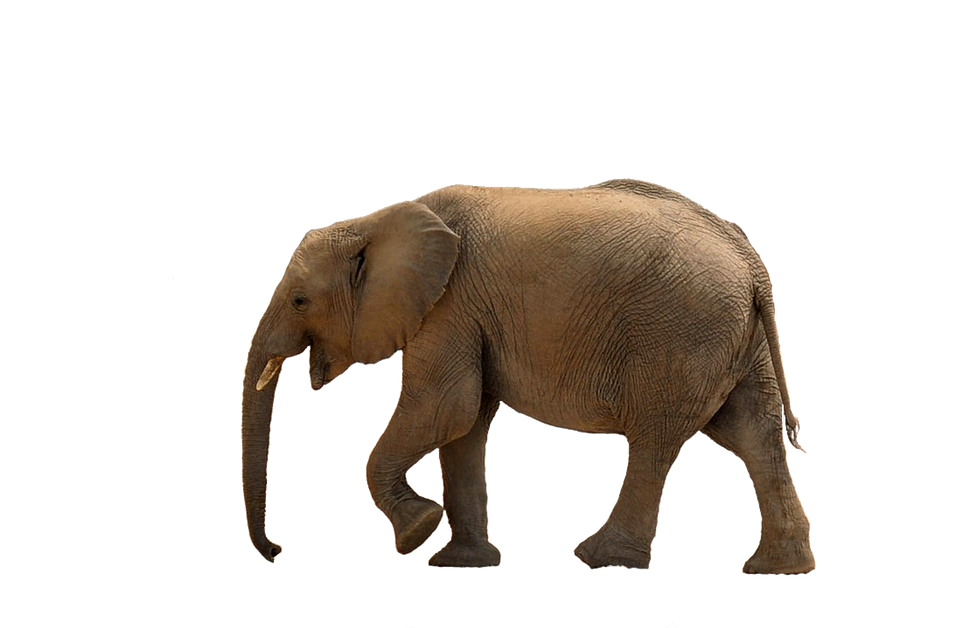
\includegraphics[width=5cm]{images/elephant}};
	\node[xshift=-2cm,yshift=-8.5cm] at (current page.north east) {\footnotesize{\textit{Image source: Pixabay}}};
	\end{tikzpicture}
\end{frame}

\note{
	\begin{itemize}
		\item the elephant in the room
		\item machine learning algorithms tend to create nonlinear, 
		\item non-monotonic, 
		\item non-polynomial, 
		\item and even non-continuous functions 
		\item that approximate the relationship between independent and dependent variables in a data set
		\item most ML algorithms model high-degree interactions between variables (meaning the effect of combining many?i.e., more than two or three?variables together)
	\end{itemize}

	\begin{itemize}
		\item When working with data you should be asking yourselves some very hard questions: 
		\item do I understand my data? 
		\item Do I understand the model and answers my machine learning algorithm is giving me? 
		\item And do I trust these answers? 
		\item Unfortunately, the complexity that bestows the extraordinary predictive abilities on machine learning algorithms also makes the answers the algorithms produce hard to understand, 
		\item and maybe even hard to trust.
		\item almost by definition one cannot really understand a good model
		\item difficulties in interpretation still present a barrier for the widespread, practical use of ML
		\item trusting models and results is a general requirement for good (data) science
		\item we want to understand them as well as possible
	\end{itemize}
}

%%%%%%%%%%%%%%%%%%%%%
%	SECTION
%	A quick recap of ML basics
%%%%%%%%%%%%%%%%%%%%%

\section{A quick recap of ML basics}

\begin{frame}
	\frametitle{Machine learning}

	\begin{itemize}
		\item artificial intelligence (AI)
		\item data-driven
		\item algorithms \alert{learn} by being trained on observed data...
		\item ... and \alert{predict unknown data}
		\item ML concepts are not new, but the increase in computational capacity has made them more accessible
	\end{itemize}
	
	\begin{block} {}	
		\begin{center}
			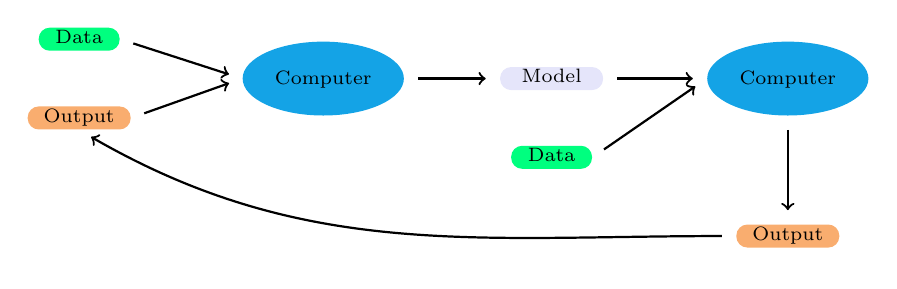
\begin{tikzpicture}
			\scriptsize
			\node[rectangle, rounded corners, text height=1ex,text depth=0ex,align=center,text width=3em,text centered,minimum height=1em, fill = SpringGreen] (Data) at (0,0) {Data};
			\node[rectangle, rounded corners, text height=1ex,text depth=0ex,align=center,text width=4em,text centered,minimum height=1em, fill = Lavender] (Model) at (6,-0.5) {Model};
			\node[ellipse, text height=3ex,text depth=1.5ex,align=center,text width=4.5em,text centered,minimum height=3em, fill = Cerulean] (Computer) at (3.1,-0.5) {Computer};
			\node[rectangle, rounded corners, text height=1ex,text depth=0ex,align=center,text width=4em,text centered,minimum height=1em, fill = Apricot] (Output) at (0,-1) {Output};
			\node[ellipse, text height=3ex,text depth=1.5ex,align=center,text width=4.5em,text centered,minimum height=3em, fill = Cerulean] (Computer2) at (9,-0.5) {Computer};
			\node[rectangle, rounded corners, text height=1ex,text depth=0ex,align=center,text width=4em,text centered,minimum height=1em, fill = Apricot] (Output2) at (9,-2.5) {Output};
			\node[rectangle, rounded corners, text height=1ex,text depth=0ex,align=center,text width=3em,text centered,minimum height=1em, fill = SpringGreen] (Data2) at (6,-1.5) {Data};
			
			\draw[->,thick,shorten >=5pt,shorten <=5pt] (Data.east) -- (Computer.west);
			\draw[->,thick,shorten >=5pt,shorten <=5pt] (Output.east) -- (Computer.west);
			\draw[->,thick,shorten >=5pt,shorten <=5pt] (Computer.east) -- (Model.west);
			\draw[->,thick,shorten >=5pt,shorten <=5pt] (Model.east) -- (Computer2.west);
			\draw[->,thick,shorten >=5pt,shorten <=5pt] (Computer2.south) -- (Output2.north);
			\draw[->,thick,shorten >=5pt,shorten <=5pt] (Data2.east) -- (Computer2.west);
			\draw[->,thick,shorten >=5pt,shorten <=5pt] (Output2.west) to [out=180,in=330] (Output.south);
			\end{tikzpicture}
		\end{center}
	\end{block}
\end{frame}

\begin{frame}
	\frametitle{Supervised vs Unsupervised algorithms}

	\begin{columns}
		
		\column{0.5\textwidth}
	
	\begin{block}{}
		\centering
		\alert{Supervised}
	\end{block}

	\begin{center}
		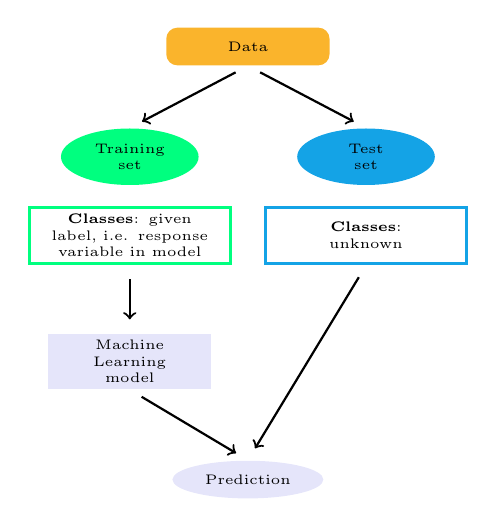
\begin{tikzpicture}
		\tiny
		\node[rectangle, rounded corners, align=center,text width=8em,text centered,minimum height=2em, fill = Dandelion] (select) at (2.5,-3) {Data};
		
		\node[ellipse,align=center,text width=4.5em,text centered,minimum height=3em, fill = SpringGreen] (training) at (1,-4.4) {Training set};
		
		\node[rectangle, align=center,text width=10em,text centered,minimum height=3em, draw = SpringGreen, very thick] (class1) at (1,-5.4) {\textbf{Classes}: given label, i.e. response variable in model};
		
		\node[ellipse,align=center,text width=4.5em,text centered,minimum height=3em, fill = Cerulean] (test) at (4,-4.4) {Test \\ set};
		
		\node[rectangle, align=center,text width=10em,text centered,minimum height=3em, draw = Cerulean, very thick] (class2) at (4,-5.4) {\textbf{Classes}: \\ unknown};
		
		\node[rectangle, align=center,text width=8em,text centered,minimum height=2em, fill = Lavender] (rf) at (1,-7.0) {Machine \\ Learning \\ model};
		
		\node[ellipse,align=center,text width=5em,text centered,minimum height=2em, fill = Lavender] (prediction) at (2.5,-8.5) {Prediction};
		
		\draw[->,thick,shorten >=5pt,shorten <=5pt] (select.south) -- (training.north);
		\draw[->,thick,shorten >=5pt,shorten <=5pt] (select.south) -- (test.north);
		
		\draw[->,thick,shorten >=5pt,shorten <=5pt] (class1.south) -- (rf.north);
		\draw[->,thick,shorten >=5pt,shorten <=5pt] (class2.south) -- (prediction.north);
		
		\draw[->,thick,shorten >=5pt,shorten <=5pt] (rf.south) -- (prediction.north);
		\end{tikzpicture}
		
		\footnotesize{\textit{}}
	\end{center}

	\column{0.5\textwidth}
	
	\begin{block}{}
		\centering
		\alert{Unsupervised}
	\end{block}

	\centering
	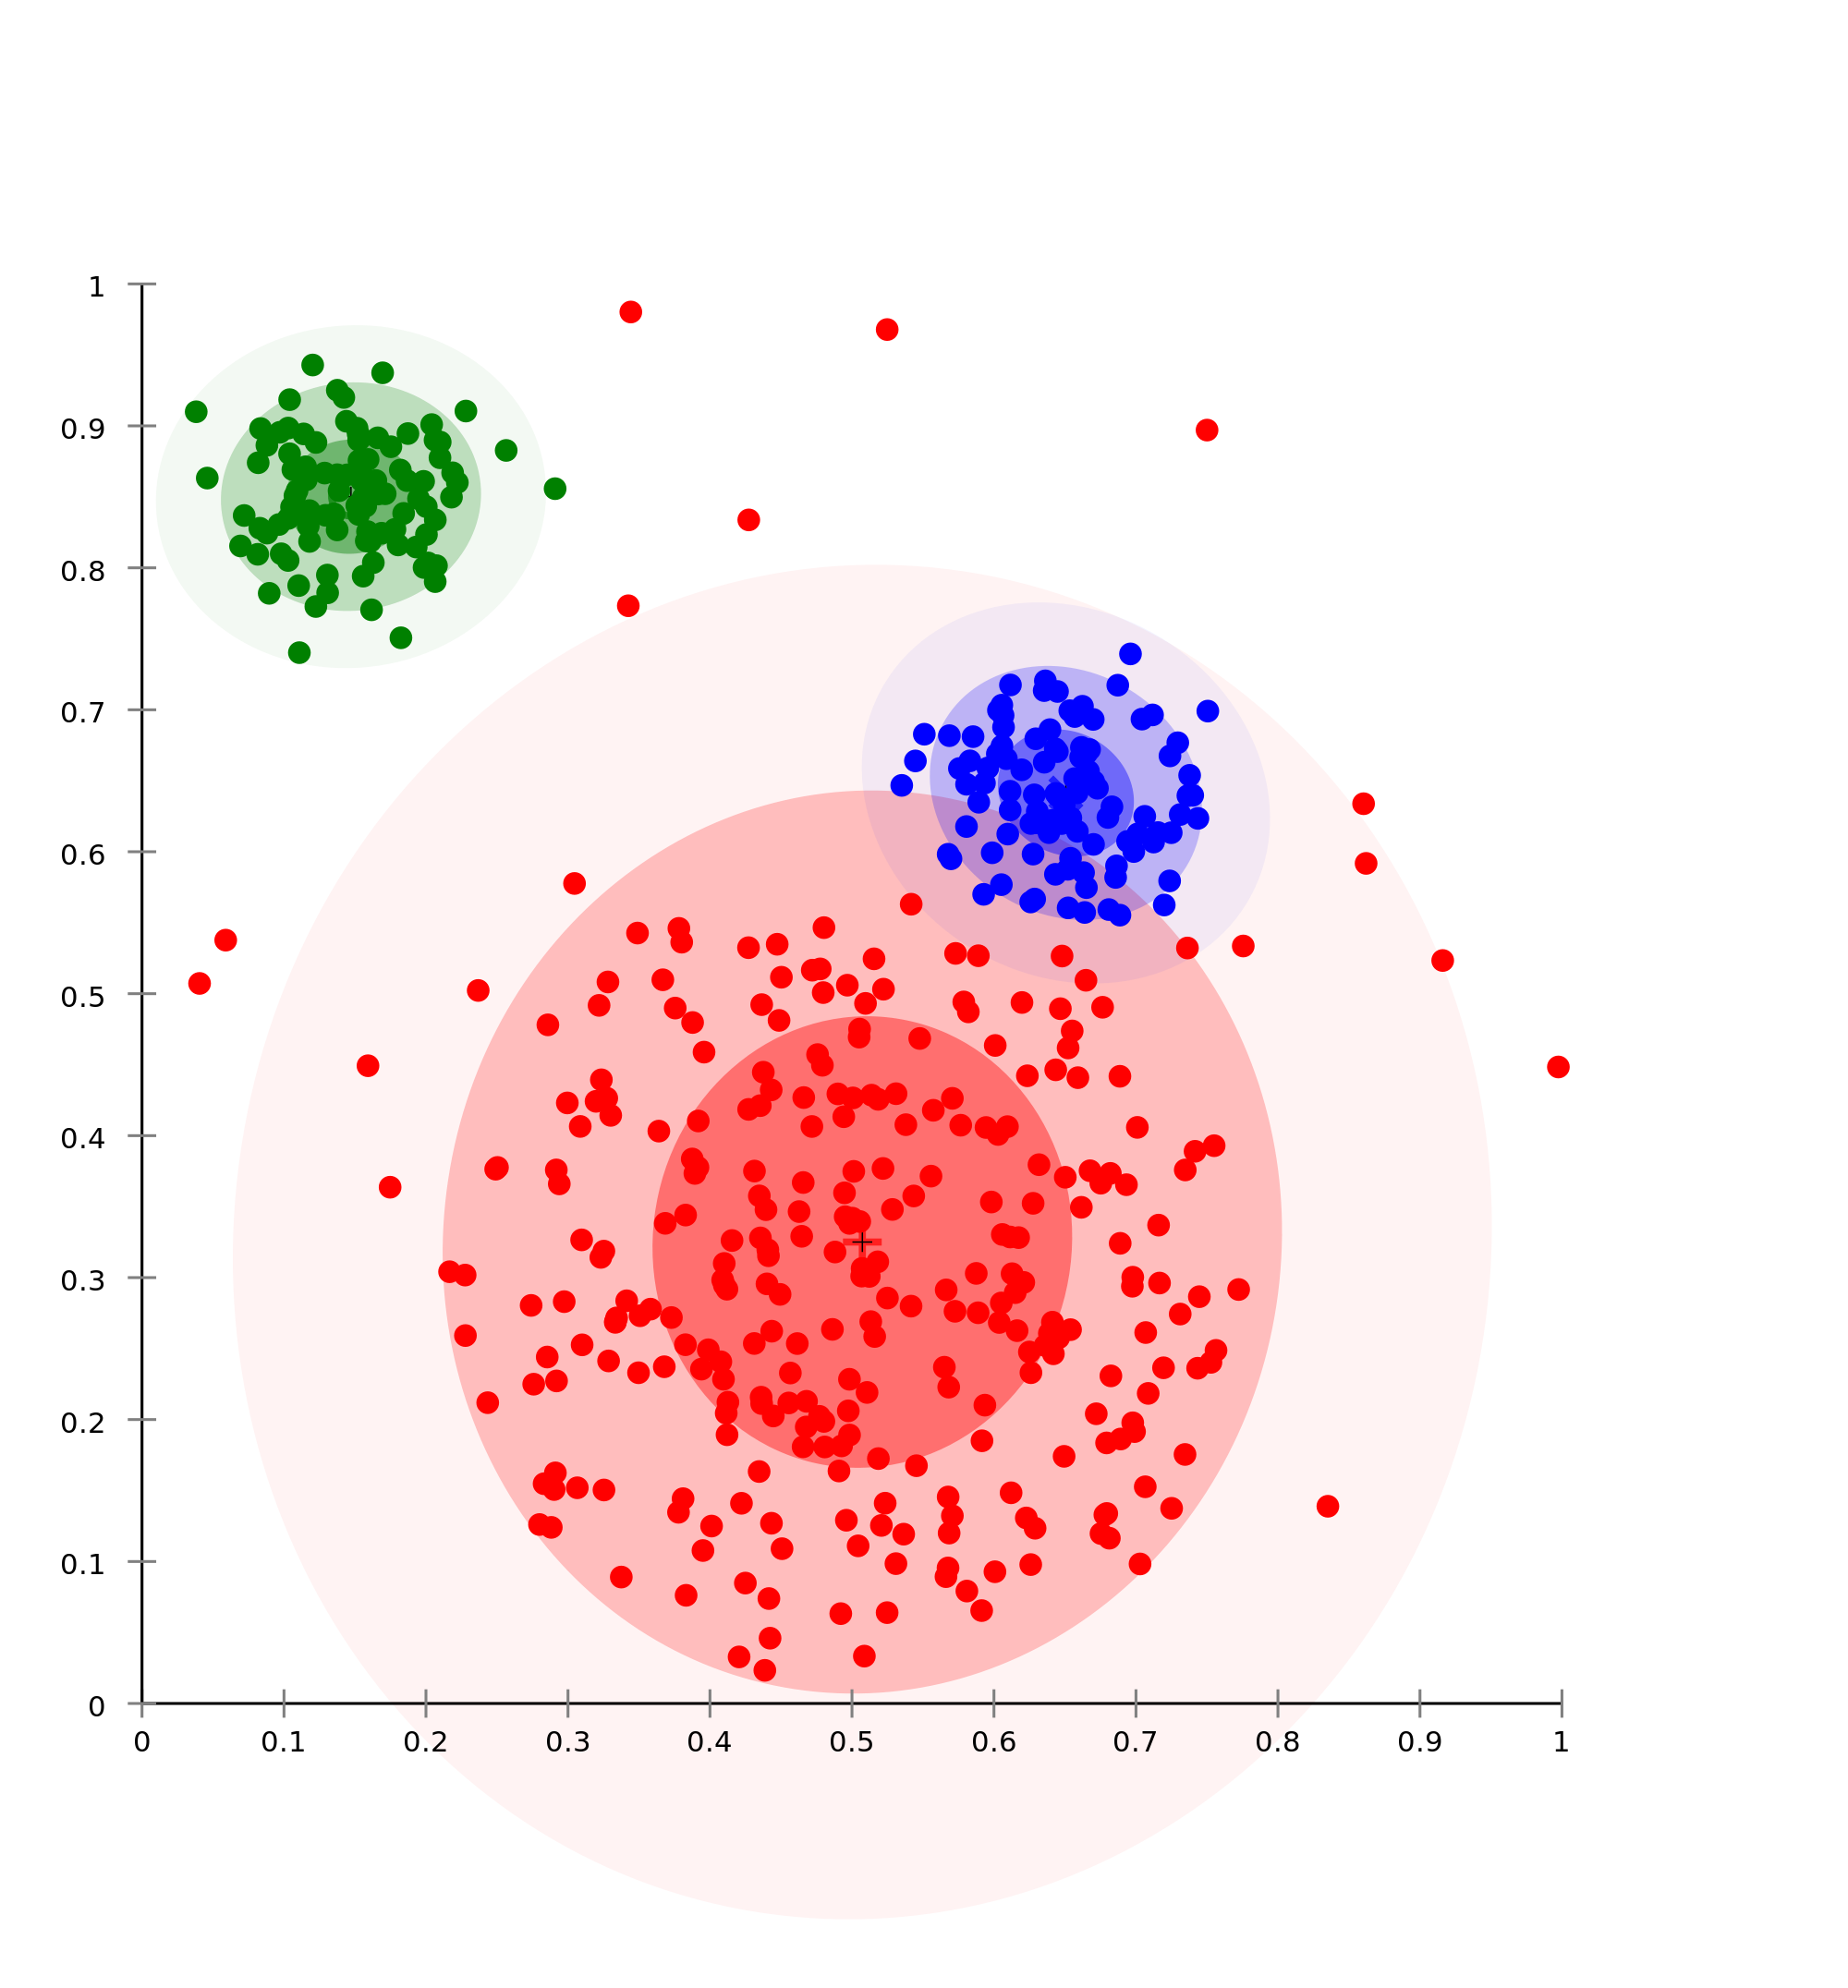
\includegraphics[width=0.5\textwidth]{images/clustering1}
	
	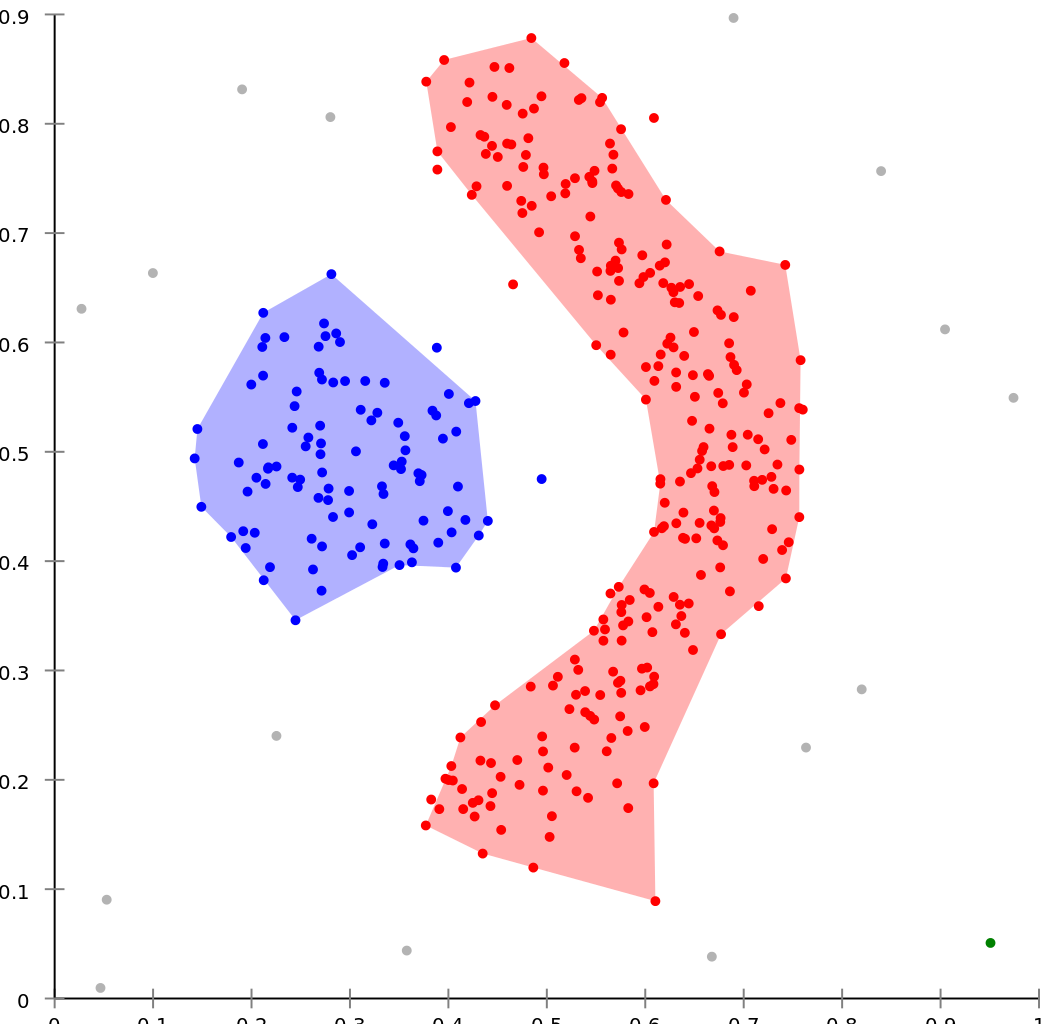
\includegraphics[width=0.5\textwidth]{images/clustering2}
	
	\footnotesize{\textit{Wikipedia}}
	
	\end{columns}
\end{frame}

\note{
	\begin{itemize}
		\item Unsupervised:
		\item no input!
		\item matrix decomposition methods, e.g. nonnegative matrix factorization
		\item pattern recognition
		\item clusters data into different groups
		\item able to recover biomarkers of disease and toxicity
	\end{itemize}

	\begin{itemize}
		\item Supervised
		\item classification labels are given
		\item e.g. support vector machine
	\end{itemize}

	\begin{itemize}
	\item Semi-supervised:
	\item a little bit of input, like how many classes to find
	\end{itemize}

	Here, I will focus on supervised learning!
}


\begin{frame}
	\frametitle{Classification vs Regression}

		\begin{columns}
		
		\column{0.5\textwidth}
		
				\begin{block}{}
			\centering
			\alert{Regression} \\
			e.g. weight loss
		\end{block}
		
		\begin{center}
			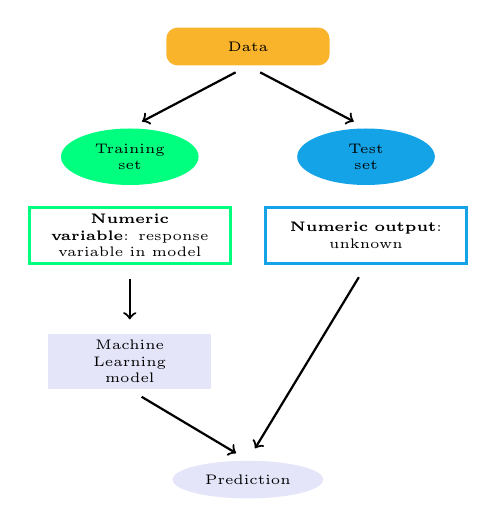
\begin{tikzpicture}
			\tiny
			\node[rectangle, rounded corners, align=center,text width=8em,text centered,minimum height=2em, fill = Dandelion] (select) at (2.5,-3) {Data};
			
			\node[ellipse,align=center,text width=4.5em,text centered,minimum height=3em, fill = SpringGreen] (training) at (1,-4.4) {Training set};
			
			\node[rectangle, align=center,text width=10em,text centered,minimum height=3em, draw = SpringGreen, very thick] (class1) at (1,-5.4) {\textbf{Numeric \\ variable}: response variable in model};
			
			\node[ellipse,align=center,text width=4.5em,text centered,minimum height=3em, fill = Cerulean] (test) at (4,-4.4) {Test \\ set};
			
			\node[rectangle, align=center,text width=10em,text centered,minimum height=3em, draw = Cerulean, very thick] (class2) at (4,-5.4) {\textbf{Numeric output}: \\ unknown};
			
			\node[rectangle, align=center,text width=8em,text centered,minimum height=2em, fill = Lavender] (rf) at (1,-7.0) {Machine \\ Learning \\ model};
			
			\node[ellipse,align=center,text width=5em,text centered,minimum height=2em, fill = Lavender] (prediction) at (2.5,-8.5) {Prediction};
			
			\draw[->,thick,shorten >=5pt,shorten <=5pt] (select.south) -- (training.north);
			\draw[->,thick,shorten >=5pt,shorten <=5pt] (select.south) -- (test.north);
			
			\draw[->,thick,shorten >=5pt,shorten <=5pt] (class1.south) -- (rf.north);
			\draw[->,thick,shorten >=5pt,shorten <=5pt] (class2.south) -- (prediction.north);
			
			\draw[->,thick,shorten >=5pt,shorten <=5pt] (rf.south) -- (prediction.north);
			\end{tikzpicture}
		\end{center}
		
		\column{0.5\textwidth}
		
		\pause
		
		\begin{block}{}
			\centering
			\alert{Classification} \\
			e.g. healthy vs disease
		\end{block}
		
		\begin{center}
			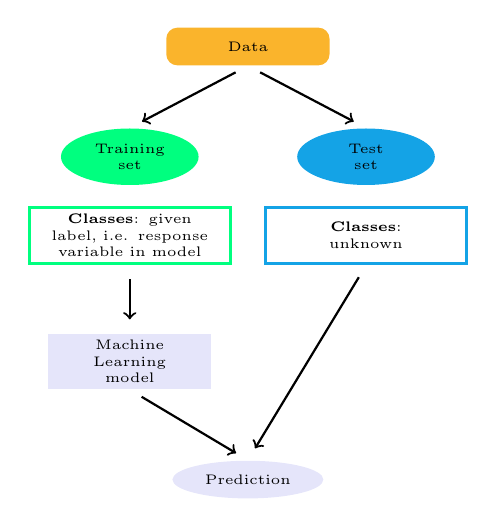
\begin{tikzpicture}
			\tiny
			\node[rectangle, rounded corners, align=center,text width=8em,text centered,minimum height=2em, fill = Dandelion] (select) at (2.5,-3) {Data};
			
			\node[ellipse,align=center,text width=4.5em,text centered,minimum height=3em, fill = SpringGreen] (training) at (1,-4.4) {Training set};
			
			\node[rectangle, align=center,text width=10em,text centered,minimum height=3em, draw = SpringGreen, very thick] (class1) at (1,-5.4) {\textbf{Classes}: given label, i.e. response variable in model};
			
			\node[ellipse,align=center,text width=4.5em,text centered,minimum height=3em, fill = Cerulean] (test) at (4,-4.4) {Test \\ set};
			
			\node[rectangle, align=center,text width=10em,text centered,minimum height=3em, draw = Cerulean, very thick] (class2) at (4,-5.4) {\textbf{Classes}: \\ unknown};
			
			\node[rectangle, align=center,text width=8em,text centered,minimum height=2em, fill = Lavender] (rf) at (1,-7.0) {Machine \\ Learning \\ model};
			
			\node[ellipse,align=center,text width=5em,text centered,minimum height=2em, fill = Lavender] (prediction) at (2.5,-8.5) {Prediction};
			
			\draw[->,thick,shorten >=5pt,shorten <=5pt] (select.south) -- (training.north);
			\draw[->,thick,shorten >=5pt,shorten <=5pt] (select.south) -- (test.north);
			
			\draw[->,thick,shorten >=5pt,shorten <=5pt] (class1.south) -- (rf.north);
			\draw[->,thick,shorten >=5pt,shorten <=5pt] (class2.south) -- (prediction.north);
			
			\draw[->,thick,shorten >=5pt,shorten <=5pt] (rf.south) -- (prediction.north);
			\end{tikzpicture}
		\end{center}
		
	\end{columns}
\end{frame}

\note{
	\begin{itemize}
		\item Supervised learning!
		\item Your learning algorithm seeks a function from inputs to the respective targets. 
		\item If the targets are expressed in some classes, it is called classification problem. 
		\item Alternatively, if the target space is continuous, it is called regression problem.
	\end{itemize}

	\begin{itemize}
		\item Functions created by linear regression algorithms are probably the most interpretable class of models.
		\item For this reason, linear models were the go-to applied predictive modeling tool for decades, 
		\item even though it usually meant giving up a couple points on the accuracy scale. 
		\item These models will be referred to here as 'linear and monotonic',
		\item meaning that for a change in any given independent variable, the response function changes at a defined rate, 
		\item in only one direction, and at a magnitude represented by a readily available coefficient
	\end{itemize}

	\begin{itemize}
		\item Most machine learning algorithms create nonlinear, non-monotonic response functions. 
		\item This class of functions is the most difficult to interpret, as they can change in a positive and negative direction and at a varying rate for any change in an independent variable. 
		\item Typically, the only standard interpretability measure these functions provide are relative variable importance measures
	\end{itemize}
}


\begin{frame}
	\frametitle{Features}
	
	\begin{columns}
		\column{0.5\textwidth}
	
	\begin{itemize}
	\item Features are the variables used for model training.
	\item Using the right features is crucial.
	\end{itemize}

		\vspace{0.5cm}

	\begin{itemize}
		\item \alert{More is not necessarily better (overfitting)!}
	\end{itemize}
	
		\vspace{0.5cm}

	\begin{itemize}
		\item feature selection
		\item feature extraction/ engineering
	\end{itemize}

	\column{0.5\textwidth}
	\begin{tikzpicture}[remember picture,overlay]
	\node[xshift=-3cm,yshift=4.5cm] at (current page.south east) {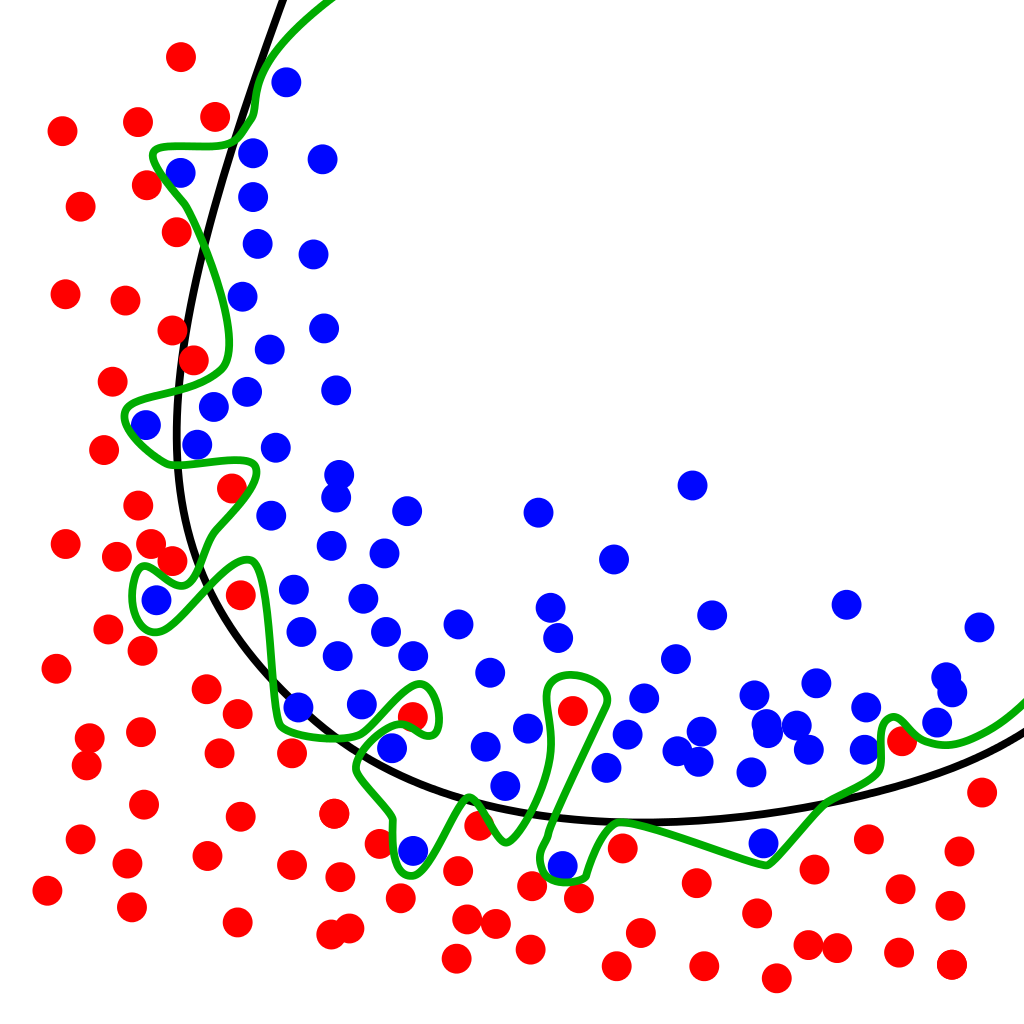
\includegraphics[width=5cm]{images/Overfitting}};
	\node[xshift=-1.5cm,yshift=1.5cm] at (current page.south east) {{\footnotesize \textit{Wikipedia}}};
	\end{tikzpicture}
	
	\end{columns}
\end{frame}

\note{
	\begin{itemize}
		\item Machine learning uses so called features (i.e. variables or attributes) to generate predictive models
		\item Using a suitable combination of features is essential for obtaining high precision and accuracy. 
		\item Because too many (unspecific) features pose the problem of overfitting the model, we generally want to restrict the features in our models to those, that are most relevant for the response variable we want to predict. 
		\item Using as few features as possible will also reduce the complexity of our models, which means it needs less time and computer power to run and is easier to understand. 
		\item Sometimes extraction of salient structure in the data that is more informative than the raw data itself (the feature extraction problem)
	\end{itemize}
}

\begin{frame}
	\frametitle{Training, (cross-) validation and test data}
	
\end{frame}

\note{
	Decide cross validation strategy - To avoid overfitting, make sure you've set up a cross validation strategy in early stages. A nice CV strategy will help you get reliable score on leaderboard.
	
	preventing overfitting, we want our models to be generalizable
	
	Cross validation means that from my main set, I create RANDOMLY 2 sets. I built (train) my algorithm with the first one (let?s call it training set) and score the other (let?s call it validation set). I repeat this process multiple times and always check how my model performs on the test set in respect to the metric I want to optimize.
	
	The process may look like:
	
	For 10 (you choose how many X) times
	Split the set in training (50%-90% of the original data)
	And validation (50%-10%  of the original data)
	Then fit the algorithm on the training set
	Score the validation set.
	Save the result of that scoring in respect to the chosen metric.
	Calculate the average of these 10 (X) times. That how much you expect this score in real life and is generally a good estimate.
	Remember to use a SEED to be able to replicate these X splits
	Other things to consider is Kfold and stratified KFold . Read here. For time sensitive data, make certain you always the rule of having past predicting future when testings.
}
\begin{frame}
	\frametitle{Hyper Parameter Tuning}
	
\end{frame}

\note{
	Grid Search
	
	Start hyper parameter tuning - Once CV is at place, try improving model's accuracy using hyper parameter tuning. It further includes the following steps:
	Data transformations: It involve steps like scaling, removing outliers, treating null values,  transform categorical variables, do feature selections, create interactions etc.
	Choosing algorithms and tuning their hyper parameters: Try multiple algorithms to understand how model performance changes.
	Saving results: From all the models trained above, make sure you save their predictions. They will be useful for ensembling.
	Combining models: At last, ensemble the models, possibly on multiple levels. Make sure the models are correlated for best results.
}

\begin{frame}[plain, c]
	
	\begin{center}
	\usebeamerfont*{frametitle} \usebeamercolor[fg]{frametitle} {\Huge \textbf{Take home messages:}}
	\end{center}

	\vspace{0.5cm}

	\begin{itemize}
		\item ...
	\end{itemize}
\end{frame}

%%%%%%%%%%%%%%%%%%%%%
%	SECTION
%	How to build ML models in R
%%%%%%%%%%%%%%%%%%%%%

\section{How to build ML models in R}

\begin{frame}
	\frametitle{Session setup}
	
	\begin{itemize}
		\item \href{http://archive.ics.uci.edu/ml/machine-learning-databases/breast-cancer-wisconsin/}{Breast Cancer Wisconsin Dataset}\footfullcite{Wolberg01121990} \\ \vspace{0.1cm}
		\includegraphics[height=2cm]{images/Needle_Biopsy.jpg}
		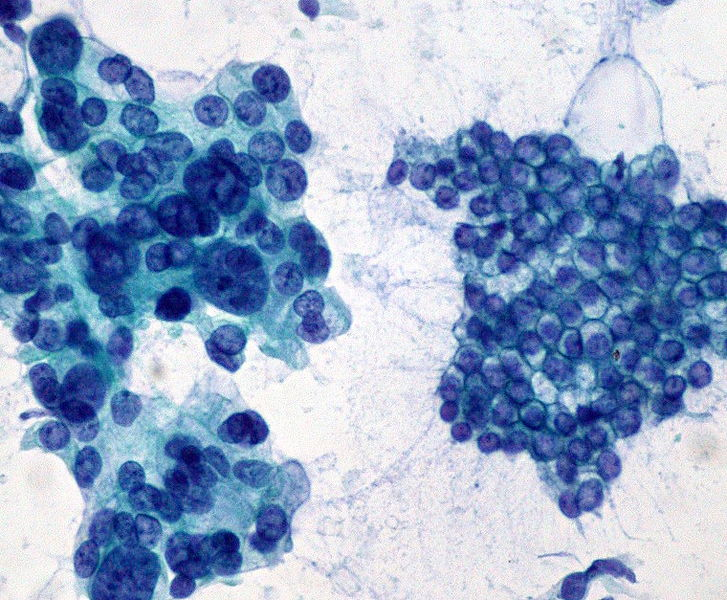
\includegraphics[height=2cm]{images/fna.jpg} \vspace{0.1cm}
		\item caret\footfullcite{caret}
		\item h2o\footfullcite{h2o}
	\end{itemize}
	
	\vspace{0.5cm}
	
	\centering
	Code will be available on \href{https://shiring.github.io}{my website} and on \href{https://github.com/ShirinG/Webinar_ML_for_disease}{Github}
	
	\begin{tikzpicture}[remember picture,overlay]
	\node[xshift=-2.3cm,yshift=-2.3cm] at (current page.north east) {
\includegraphics[width=3cm]{images/R_logo.png}};
	\end{tikzpicture}
	
\end{frame}

\note{
	\begin{itemize}
		\item This breast cancer databases was obtained from the University of Wisconsin Hospitals, Madison
		\item from Dr. William H. Wolberg
	\end{itemize}
	
	\begin{itemize}
		\item It looks at the predictor classes:
		\item malignant or
		\item benign breast mass
	\end{itemize}
	
	\begin{itemize}
		\item The features characterise cell nucleus properties
		\item and were generated from image analysis of fine needle aspirates (FNA) of breast masses:
		\item Sample ID (code number)
		\item Clump thickness
		\item Uniformity of cell size
		\item Uniformity of cell shape
		\item Marginal adhesion
		\item Single epithelial cell size
		\item Number of bare nuclei
		\item Bland chromatin
		\item Number of normal nuclei
		\item Mitosis
		\item Classes, i.e. diagnosis
	\end{itemize}
}

\begin{frame}
	\frametitle{Get to know your data}
	
	\alert{Response variable}
	\begin{itemize}
		\item Is it balanced?
	\end{itemize}
	
	\begin{columns}	
		\column{0.5\textwidth}
		\centering
		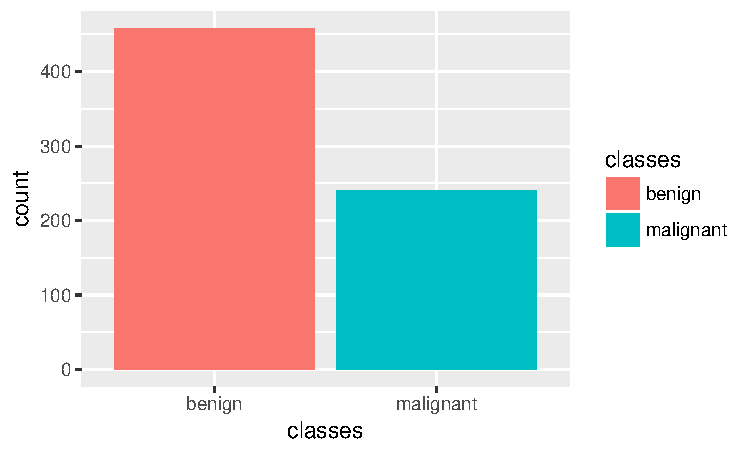
\includegraphics[width=0.9\textwidth]{webinar_code_files/figure-latex/response_classification-1.pdf}
		
		\column{0.5\textwidth}
		\centering
		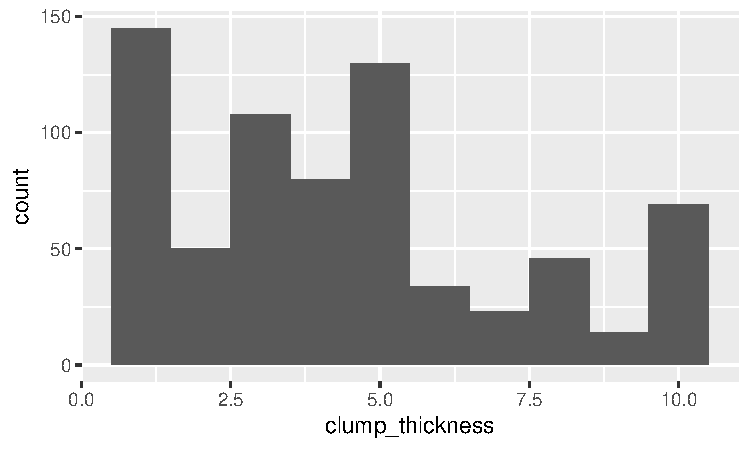
\includegraphics[width=0.9\textwidth]{webinar_code_files/figure-latex/response_regression-1.pdf}
	\end{columns}
	
		\vspace{0.5cm}

	\alert{Missing data}
	\begin{itemize}
		\item Is there missing data?
		\item Can we afford to loose data points with missing values?
		\item Or do we use imputation (and introduce additional uncertainty)?
	\end{itemize}

\end{frame}

\note{
	\begin{itemize}
		\item Understand the data
		\item Look at data types. 
		\item Check variable classes. 
		\item Create some univariate - bivariate plots to understand the nature of variables.
		\item Most important to know is the distribution: are the classes balanced?
		\item If we have unbalanced data, this will effect our model later on \\
		We would have to consider over- or undersampling.
	\end{itemize}

	\begin{itemize}
		\item Missing data
		\item If we have lots of data and few missing values, we can afford to loose these data points.
		\item If we don't have that much data though, our model will probably loose significant power if we remove the samples.
		\item In that case, we would rather introduce a certain uncertainty by imputing missing values. 
	\end{itemize}	
}

\begin{frame}
	\frametitle{Get to know your data}
	\alert{Principal Component Analysis (PCA)}
	
	\vspace{0.5cm}

	\centering
	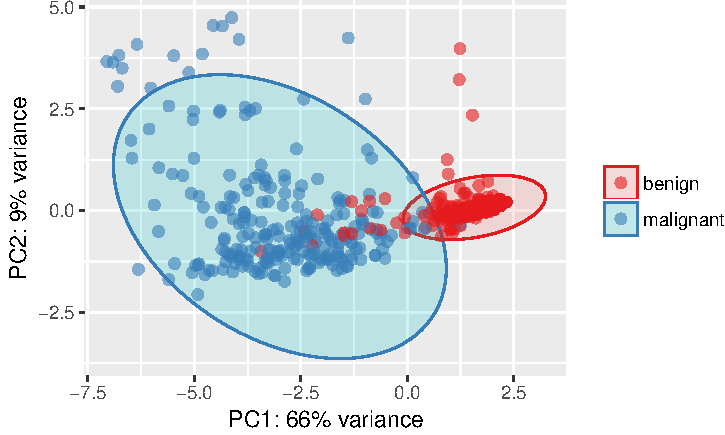
\includegraphics[width=0.9\textwidth]{webinar_code_files/figure-latex/pca-1.pdf}
\end{frame}

\begin{frame}
	\frametitle{Get to know your data}
	\alert{Principal Component Analysis (PCA)}
	
	\vspace{0.5cm}

	\centering
	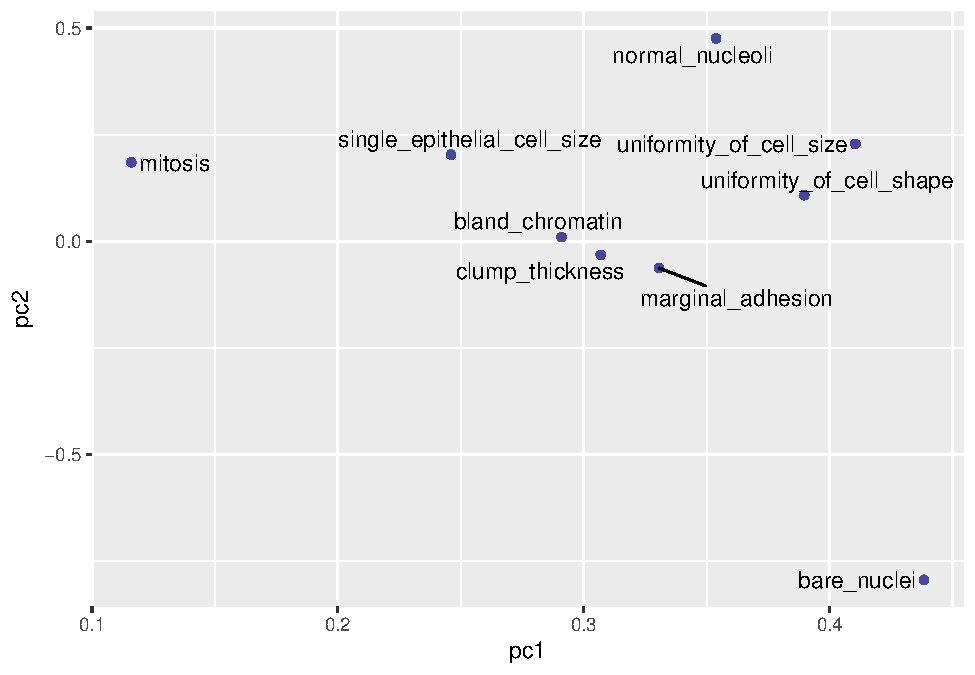
\includegraphics[width=0.8\textwidth]{webinar_code_files/figure-latex/pca_features-1.pdf}
\end{frame}

\note{
	\begin{itemize}
		\item Most real data sets are hard to see because they have many variables and many rows
		\item visualization can help when we reduce the complexity
		\item There are many techniques for projecting the rows of a data set from a usually high-dimensional original space into a more visually understandable lower-dimensional space:
		\item Principal Component Analysis (PCA)
		\item Multidimensional Scaling (MDS)
		\item t-distributed Stochastic Neighbor Embedding (t-SNE)
		\item Each of these techniques has strengths and weaknesses, but the key idea they all share is to represent the rows of a data set in a meaningful low-dimensional space. 
	\end{itemize}

	\begin{itemize}
		\item To get an idea about the dimensionality and variance of the datasets, I am first looking at PCA plots
		\item for samples and features
		\item Principal component analysis (PCA) is a statistical procedure that uses an orthogonal transformation ...
		\item ... to convert a set of observations into a set of values of linearly uncorrelated variables called principal components
		\item The first two principal components (PCs) show the two components that explain the majority of variation in the data
	\end{itemize}
}

\begin{frame}
	\frametitle{Get to know your data}
	\alert{Features}
	
	\begin{itemize}
		\item factors or numeric
		\item pre-processing
	\end{itemize}
	
	\centering
	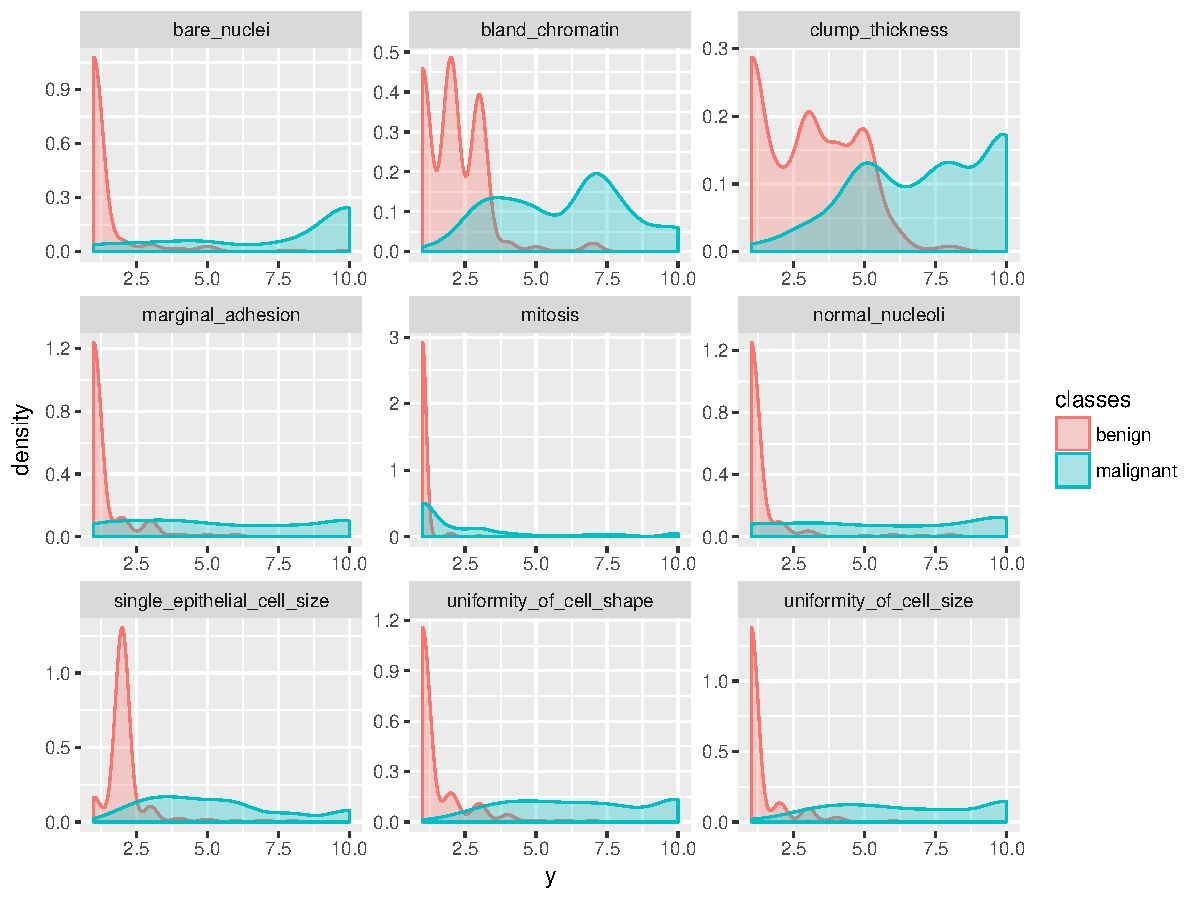
\includegraphics[width=0.7\textwidth]{webinar_code_files/figure-latex/features-1.pdf}
\end{frame}

\begin{frame}
	\frametitle{Get to know your data}
	\alert{Correlation}

	\centering
	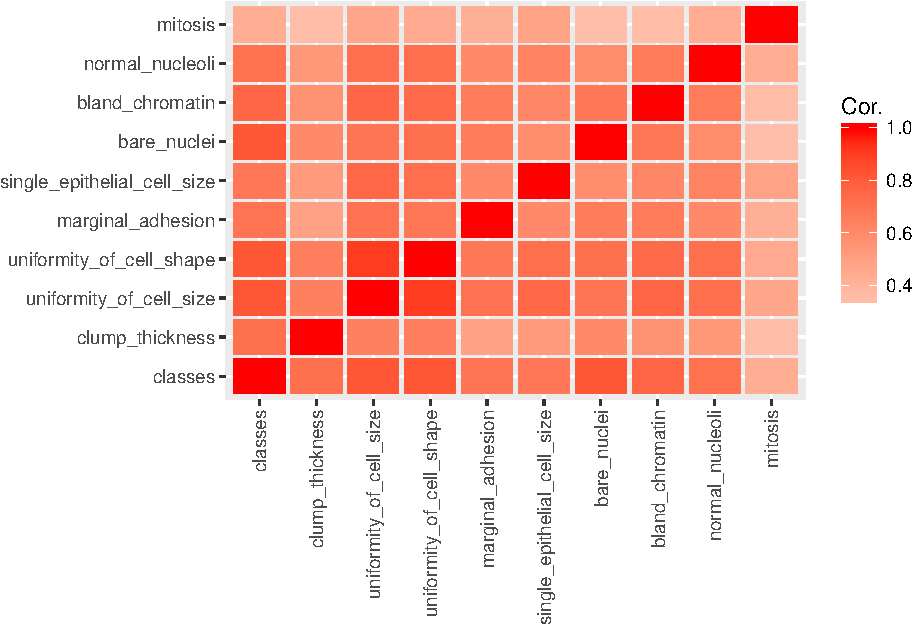
\includegraphics[width=0.9\textwidth]{webinar_code_files/figure-latex/corr_plot-1.pdf}
\end{frame}

\begin{frame}
	\frametitle{Get to know your data}
	\alert{Correlation graphs}

	\begin{center}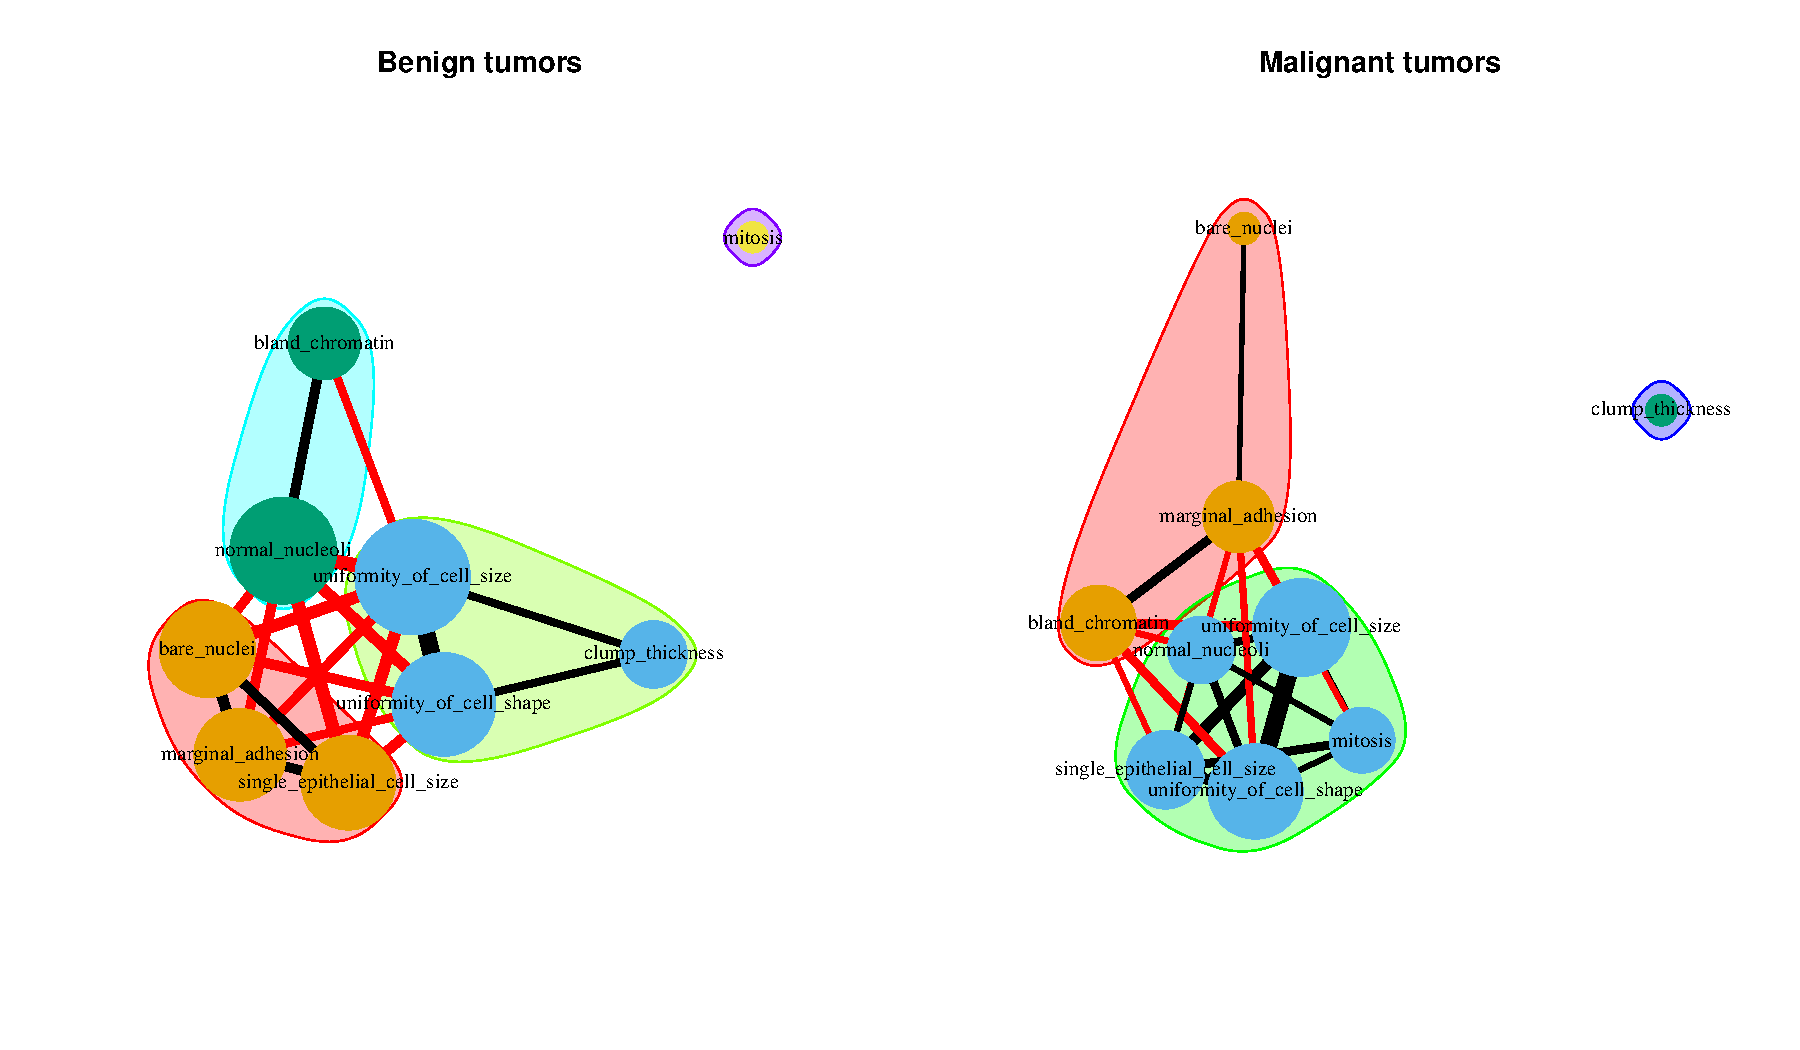
\includegraphics[width=1\textwidth]{webinar_code_files/figure-latex/cor_graph-1} \end{center}
\end{frame}

\note{
	\begin{itemize}
		\item A correlation graph is a two-dimensional representation of the relationships (correlation) in a data set
		\item Pearson correlation coefficient between features
		\item node size: sum of correlation coefficients
		\item edge width: correlation coefficient
	\end{itemize}
}


\begin{frame}
	\frametitle{Training, validation and test data}
	
	We need to split the data into training and test sets - \\
	ideally \alert{stratified} by response class.
	
	\vspace{0.5cm}

	\alert{Density distribution}
	\begin{center}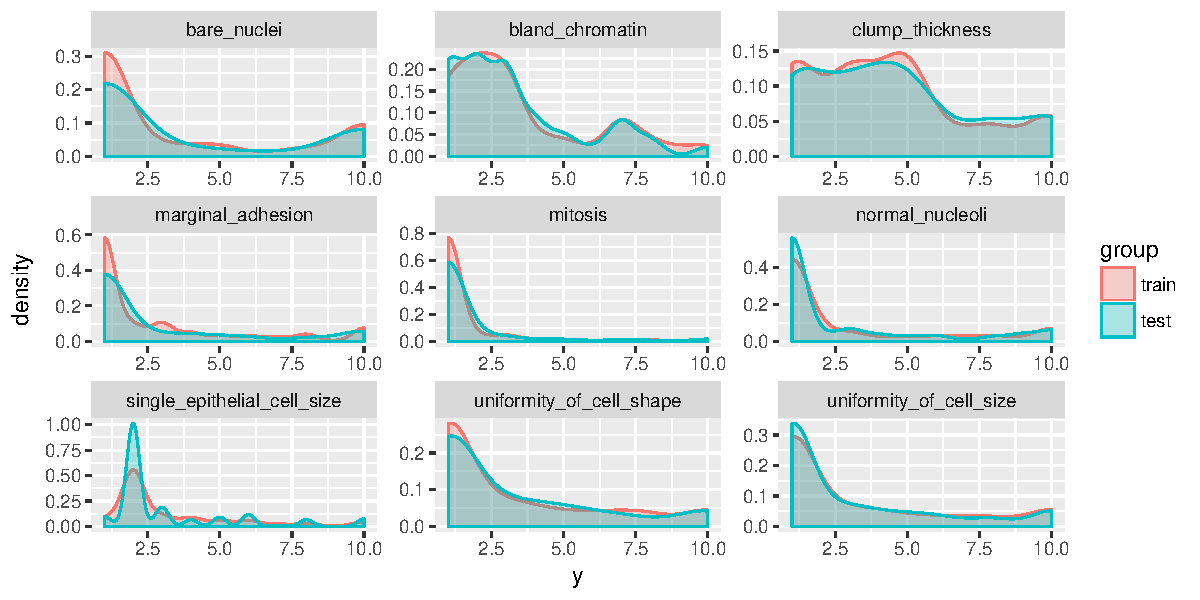
\includegraphics[width=1\textwidth]{webinar_code_files/figure-latex/distribution-1} \end{center}
\end{frame}

\note{
	For accurate predictions, density distribution should be similar in training and test data!
}

\begin{frame}
	\frametitle{Model examples}
	
	\begin{columns}
		
		\column{0.6\textwidth}
		
		\alert{Regression with Linear Models}
		\begin{itemize}
			\item e.g. Generalized Linear Models
			\item with \textsl{caret}
		\end{itemize}
		
		\vspace{0.5cm}
		
		\alert{Tree-based classification}
		\begin{itemize}
			\item Random Forest or Gradient boosting trees
			\item  with \textsl{caret}
		\end{itemize}
		
		\vspace{0.5cm}
		
		\alert{Hyper-parameter tuning}
		\begin{itemize}
			\item Grid Search
			\item  with \textsl{h2o}
		\end{itemize}
	
		\column{0.4\textwidth}
		
		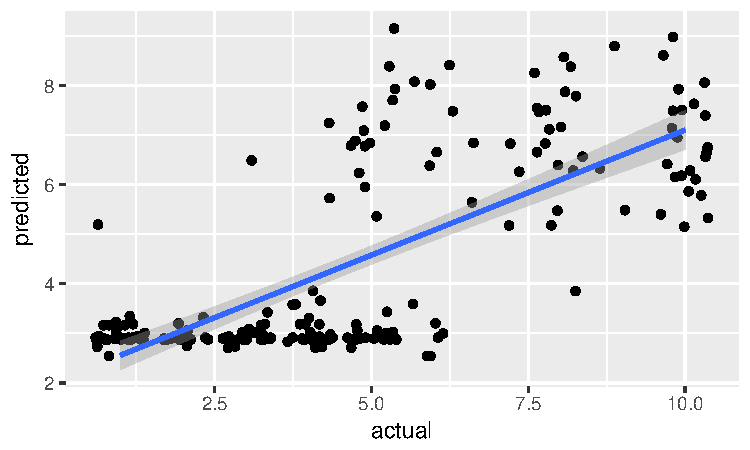
\includegraphics[width=0.9\textwidth]{webinar_code_files/figure-latex/regression_result-1.pdf}
		
		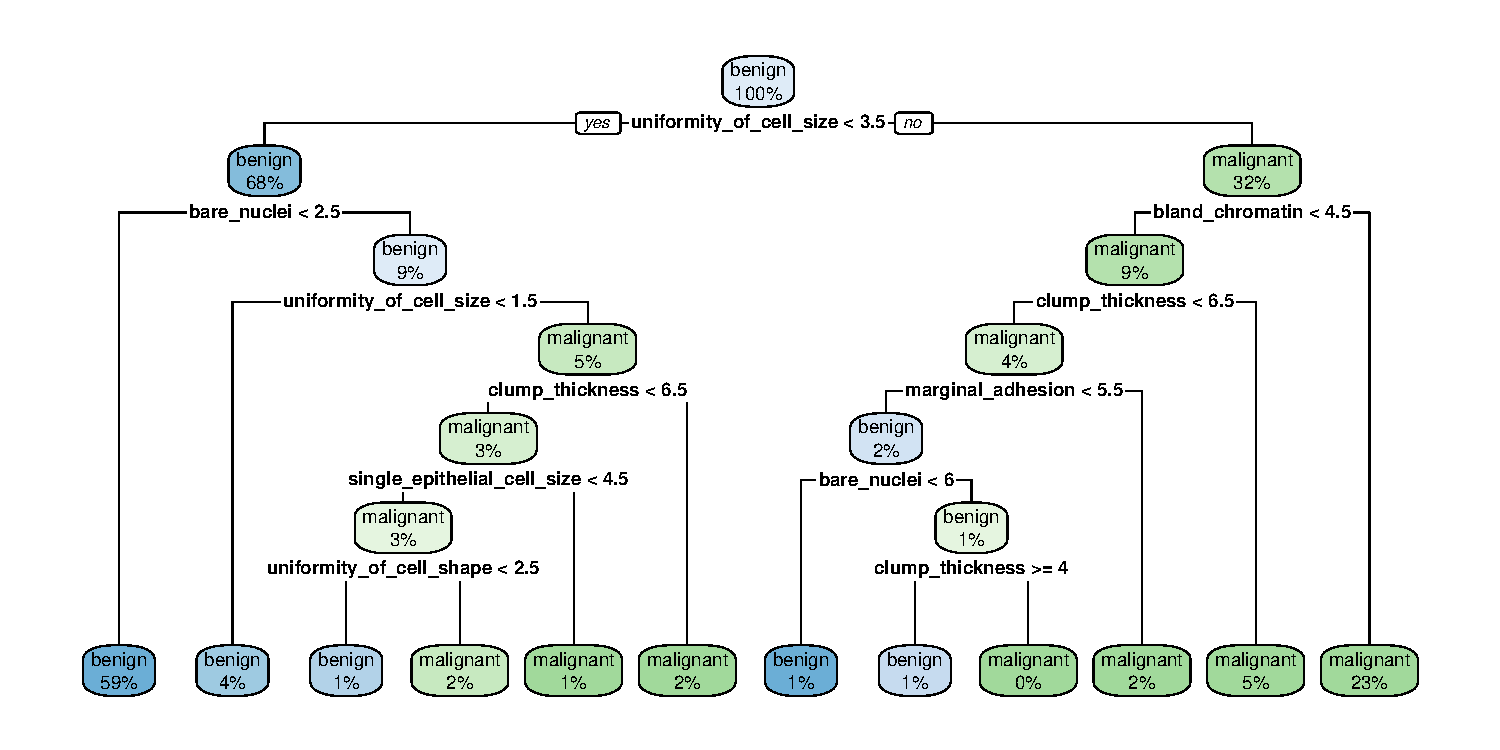
\includegraphics[width=1\textwidth]{webinar_code_files/figure-latex/decision_tree-1}
		
		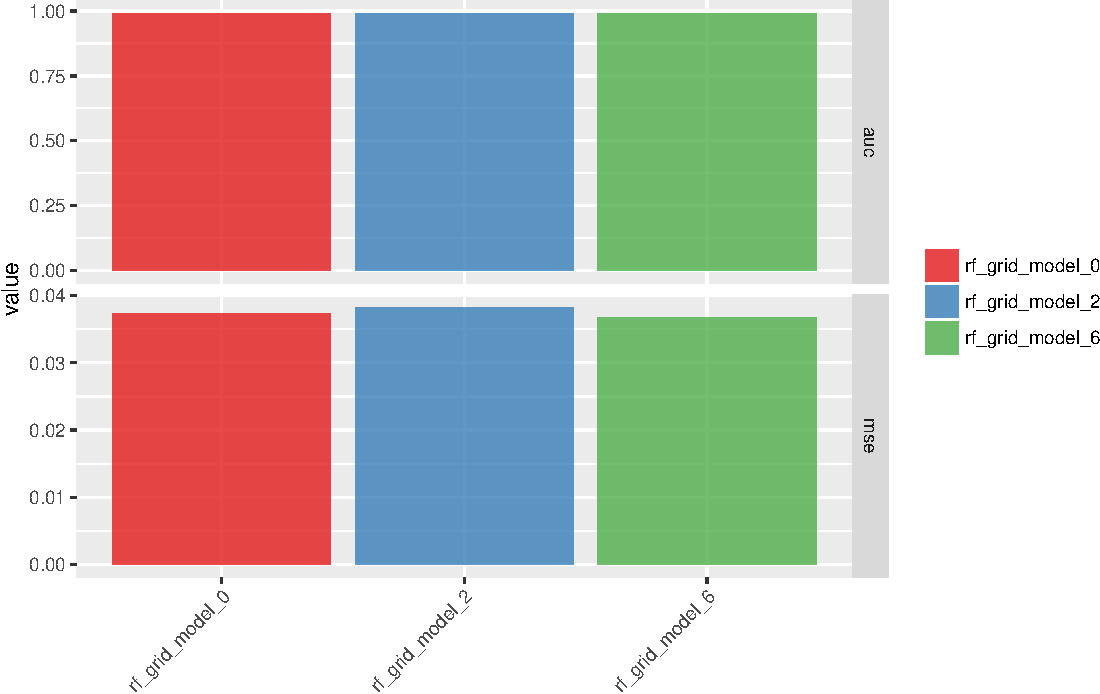
\includegraphics[width=0.9\textwidth]{webinar_code_files/figure-latex/auc_mse-1.pdf}
	\end{columns}
	
	
\end{frame}

\note{
	There are over 250 ML algorithms implemented with caret alone. I am going to focus on two of the most widely used.
	
	\begin{itemize}
		\item traditional linear models tend to create linear, monotonic, and continuous functions 
		\item Even though they?re not always the most accurate predictors, the elegant simplicity of linear models makes the results they generate easy to interpret.
	\end{itemize}

	\begin{itemize}
		\item Of course, you need quite a bit of experience and intuition to hit on a good combination of parameters.
		\item That's why it usually makes sense to do a grid search for hyper-parameter tuning. 
		\item Hyper-parameter tuning with grid search allows us to test different combinations of hyper-parameters and find one with improved accuracy.
		\item We can use the h2o.grid() function to perform a Random Grid Search (RGS). We could also test all possible combinations of parameters with Cartesian Grid or exhaustive search, but RGS is much faster when we have a large number of possible combinations and usually finds sufficiently accurate models.
		\item Based on the results of each model tested in the grid, we can choose the one with the highest accuracy or best performance for the question on hand
	\end{itemize}
}

\begin{frame}
	\frametitle{Classification with tree-based models}
	\alert{Decision trees} \\ e.g. Random Forest and gradient boosting trees
		
	\begin{center}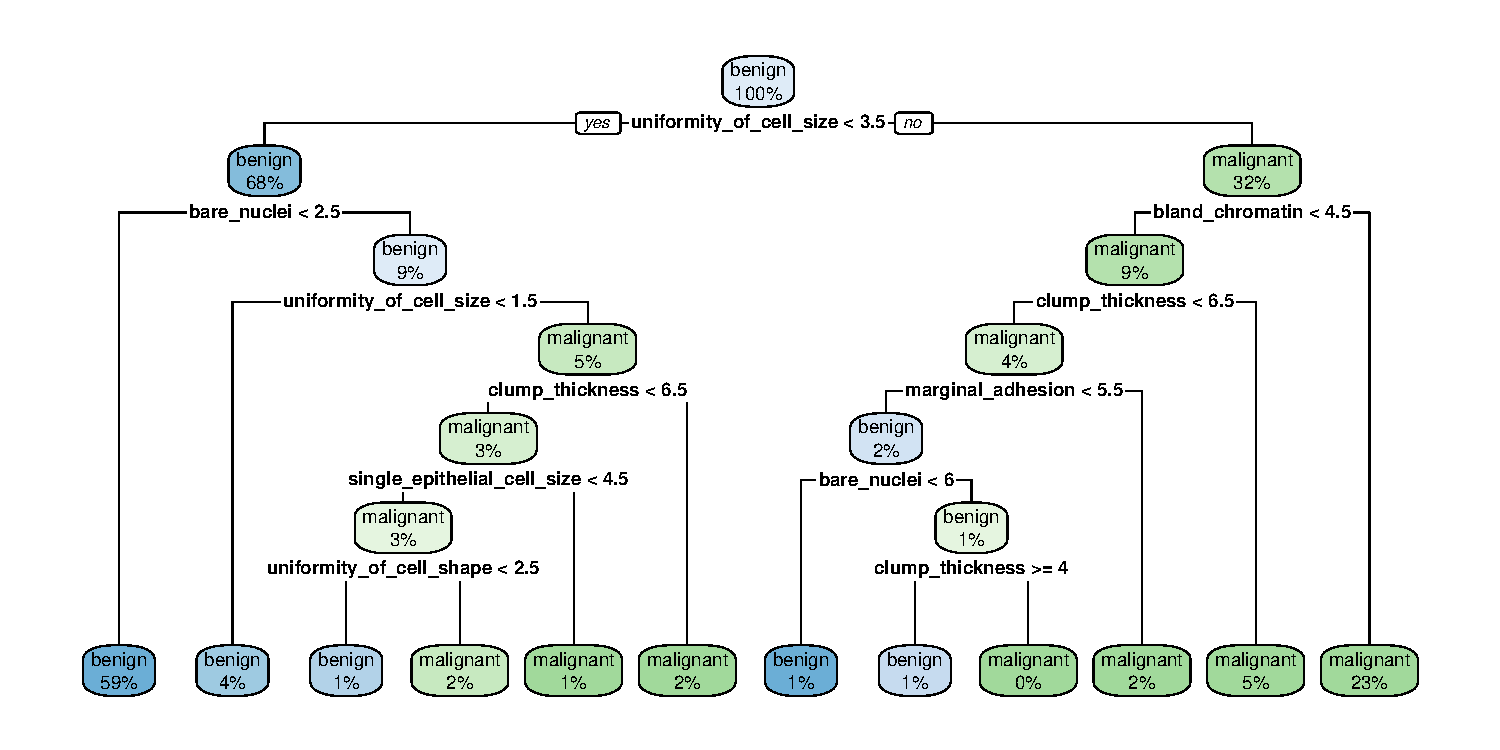
\includegraphics[width=1\textwidth]{webinar_code_files/figure-latex/decision_tree-1} \end{center}

\end{frame}

\note{
	\begin{itemize}
		\item We start with a group of samples
		\item for each sample, we assign a class: e.g. it comes from a benign or malignant tumor
		\item for each sample, we also have a number of features
		\item a decision trees separates the data at several nodes to end up with classifications at the final leaves
		\item the model learns a conditional structure of discriminative features
	\end{itemize}

	\begin{itemize}
		\item Random Forests produces multiple decision trees
		\item with some level of randomness
		\item Every node in the decision trees is a condition on a single feature, designed to split the dataset into two so that similar response values end up in the same set
		\item each tree is evaluated regarding how well it classified the samples (cross-validation)
		\item ensemble of all trees is used for prediction
		\item better generalization than individual trees
	\end{itemize}
}

\begin{frame}
	\frametitle{Feature importance}
	
	\begin{center}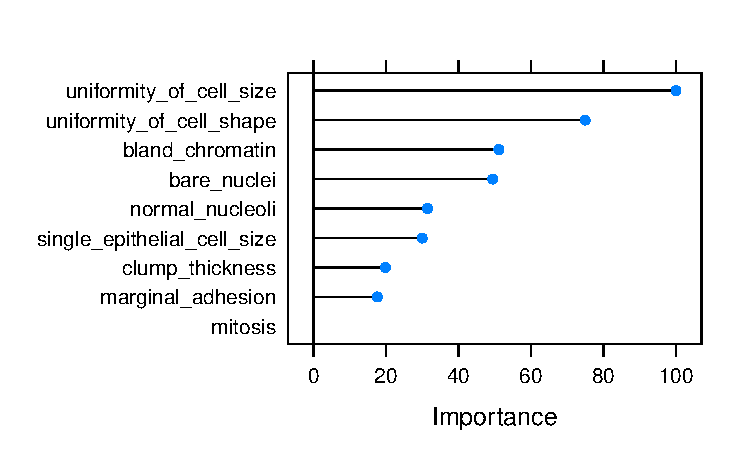
\includegraphics[width=0.8\textwidth]{webinar_code_files/figure-latex/importance_rf-1.pdf} \end{center}
\end{frame}

\note{
	\begin{itemize}
		\item Not all of the features I created will be equally important to the model. 
		\item A benefit of using ensembles of decision tree methods is that they can automatically provide estimates of feature importance from a trained predictive model.
		\item Generally, importance provides a score that indicates how useful or valuable each feature was in the construction of the decision trees within the model. 
		\item The more an attribute is used to make key decisions with decision trees, the higher its relative importance.
		\item Importance is calculated for a single decision tree by the amount that each attribute split point improves the performance measure, weighted by the number of observations the node is responsible for.
		\item The feature importances are then averaged across all of the the decision trees within the model.
		\item when training a tree, it can be computed how much each feature decreases the weighted impurity in a tree. For a forest, the impurity decrease from each feature can be averaged and the features are ranked according to this measure.
		\item 'information gain' is the measure that tells us how good a tree model is
		\item the measure based on which the (locally) optimal condition is chosen is called impurity. For classification, it is typically either Gini impurity or information gain/entropy and for regression trees it is variance
	\end{itemize}
}

%%%%%%%%%%%%%%%%%%%%%
%	SECTION
%	Evaluating model performance
%%%%%%%%%%%%%%%%%%%%%

\section{Evaluating model performance}

\begin{frame}[plain, c]
	\begin{center}
		\usebeamerfont*{frametitle} \usebeamercolor[fg]{frametitle} {\Huge \textbf{Never use the same data}}
		
		\vspace{0.2cm}
		
		\usebeamerfont*{frametitle} \usebeamercolor[fg]{frametitle} {\Huge \textbf{for evaluation that you used}}
		
		\vspace{0.2cm}
		
		\usebeamerfont*{frametitle} \usebeamercolor[fg]{frametitle} {\Huge \textbf{for training!}}
	\end{center}
\end{frame}

\note{
	\begin{itemize}
		\item Golden Rule of ML: always test model performance on indepenent data
		\item otherwise you will get overly optimistic performance measures
		\item The ultimate performance test for our model will be it's prediction accuracy on the test set it hasn't seen before.
	\end{itemize}
}


\begin{frame}
	\frametitle{Predictions on test data}
	\alert{Regression}
	
	\begin{itemize}
		\item RMSE: 1.97
		\item R\textsuperscript{2}: 0.50
	\end{itemize}
	
	\vspace{0.2cm}
	
	\centering
	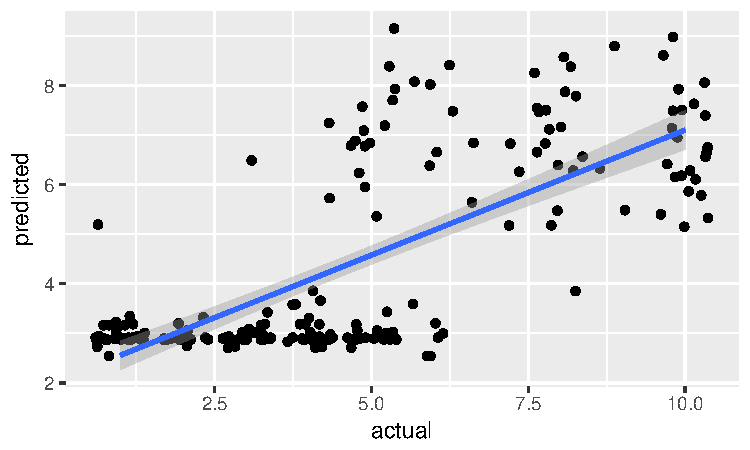
\includegraphics[width=0.5\textwidth]{webinar_code_files/figure-latex/regression_result-1.pdf}
	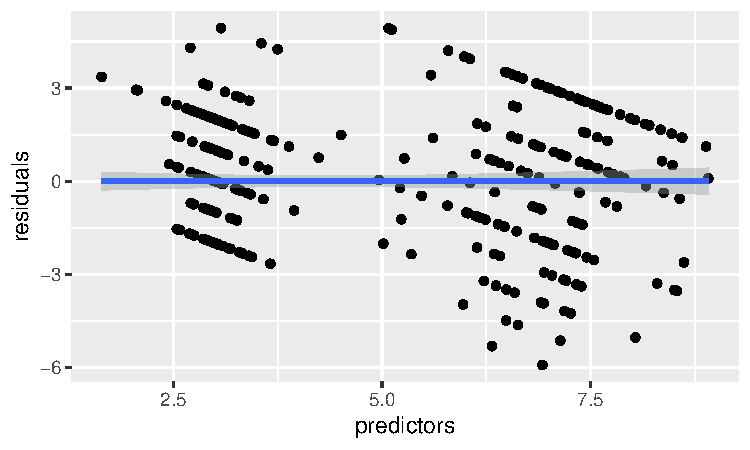
\includegraphics[width=0.5\textwidth]{webinar_code_files/figure-latex/residuals-1.pdf}
\end{frame}

\note{
	\begin{itemize}
		\item Residuals refer to the difference between the recorded value the predicted value
		\item Generally, the residuals of a well-fit model should be randomly distributed because good models will account for most phenomena in a data set, except for random error.
	\end{itemize}

	\begin{itemize}
		\item In regression analysis, the term mean squared error refers to the unbiased estimate of error variance:
		\item the residual sum of squares divided by the number of degrees of freedom
		\item RMSE is a commonly used error metric to measure the performance of regression models.
		\item in regression the predictor variable is a real number, therefore to measure the quality of the predicted value from some X algorithm you need to find some sort of difference between them. You do this by calculating the square of the error, take the mean across all test objects and take square root
		\item A small RMSE means good prediction and large means bad model.
		\item RMSE is strongly influenced by outliers!
	\end{itemize}
	
	\begin{itemize}
		\item R-squared is the ratio of explained variance to the total variance.
		\item it is a measure of how much of the variance in y is explained by the model. If R2 is close to one, then the model?s predictions mirror true outcome
	\end{itemize}
}

\begin{frame}
	\frametitle{Predictions on test data}
	\alert{Classification}
	
	\begin{columns}
	\column{0.5\textwidth}
	
	\centering
	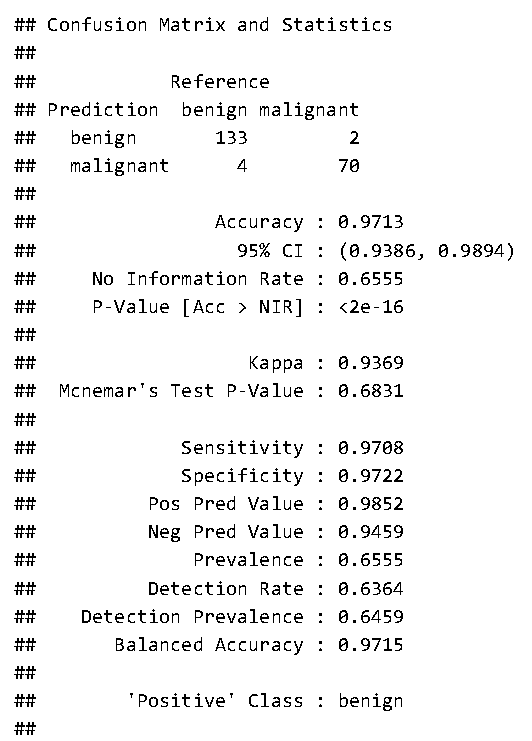
\includegraphics[width=0.9\textwidth]{images/results_matrix.pdf}
	
	\column{0.5\textwidth}
	\centering	
	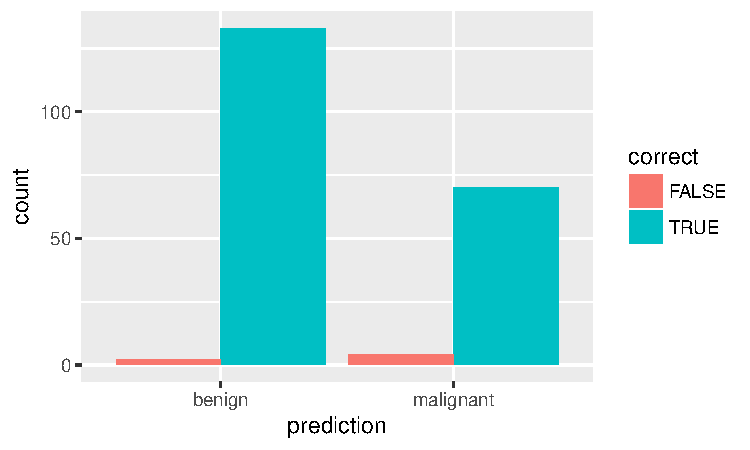
\includegraphics[width=1\textwidth]{webinar_code_files/figure-latex/results_bar_rf-1.pdf}
	
	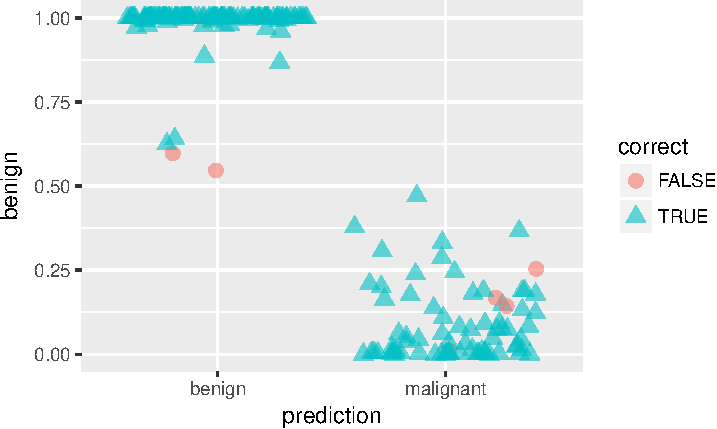
\includegraphics[width=1\textwidth]{webinar_code_files/figure-latex/results_jitter_rf-1.pdf} 
\end{columns}\end{frame}

\note{
	\begin{itemize}
		\item precision == positive predictive value: fraction of predictions that are correct
		\item positive and negative predictive values: proportions of true positive and true negative results, depend on prevalence
		\item prevalence: how often each category occurs in the population
		\item recall == sensitivity == True Positive Rate: proportion of positives that are correctly identified (e.g., the percentage of sick people who are correctly identified as having the condition).
		\item Specificity == True Negative Rate: proportion of negatives that are correctly identified (e.g., the percentage of healthy people who are correctly identified as not having the condition)
		\item Inverse Precision and Recall: Precision and Recall where positive and negative labels are exchanged
		\item detection rate == sensitivity
	\end{itemize}

	\begin{itemize}
		\item Accuracy:  weighted arithmetic mean of Precision and Recall
		\item Given a confusion matrix of classification results, the accuracy can be a misleading performance measure. Specifically,
		it may falsely suggest above-chance generalizability:
		\item in binary classification, a training set consisting of different numbers of representatives from either class may result in a classifier that is biased towards the more frequent class
		\item  this classifier may yield an optimistic accuracy estimate
		\item Balanced accuracy:  average accuracy obtained on either class. Based on a confusion matrix
	\end{itemize}

	\begin{itemize}
		\item p-value: one-sided test to see if the accuracy is better than the "no information rate"
		\item No Information Rate: the proportion of classes that you would guess right if you randomly allocated them
		\item Kappa: can have values between -1 and 1. 1 or -1 show complete agreement, zero shows complete disagreement
		\item McNemar's test: statistical test applied to 2 x 2 contingency tables to determine whether the row and column marginal frequencies are equal
	\end{itemize}
}

\begin{frame}
	\frametitle{Area Under the Curve (AUC}
	
	\centering
	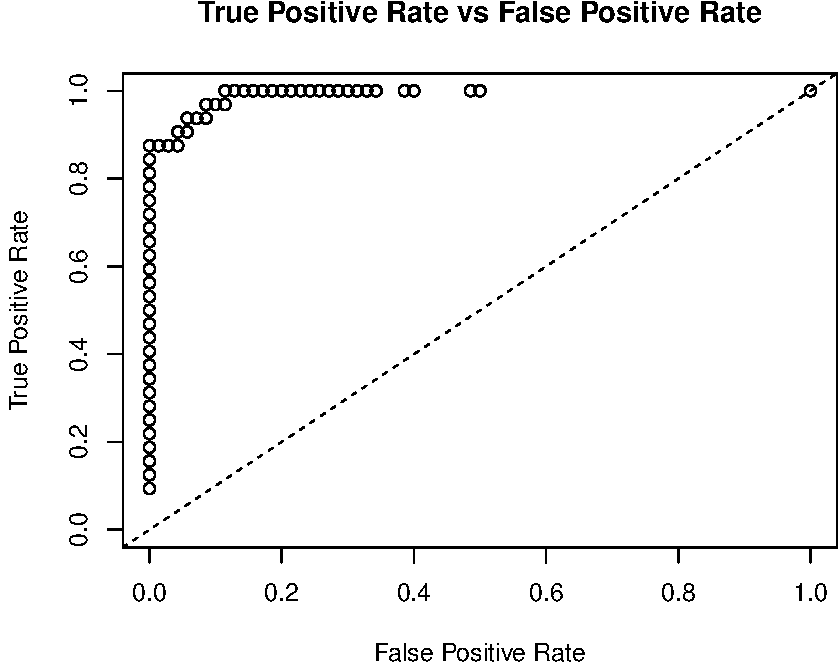
\includegraphics[width=0.8\textwidth]{webinar_code_files/figure-latex/auc_curve-1.pdf} 
\end{frame}

\note{
	\begin{itemize}
		\item AUC usually refers to area under ROC curve (mathematically known as definite integral): Receiver Operating Characteristic
		\item metric for binary classification
		\item Accuracy deals with ones and zeros, meaning you either got the class label right or you didn?t. But many classifiers are able to quantify their uncertainty about the answer by outputting a probability value.
		\item From a random classifier you can expect as many true positives as false positives. That?s the dashed line on the plot.
		\item A score for a perfect classifier would be 1
	\end{itemize}
}

\begin{frame}
	\frametitle{AUC and mean squared error (MSE)}
	
	\begin{center}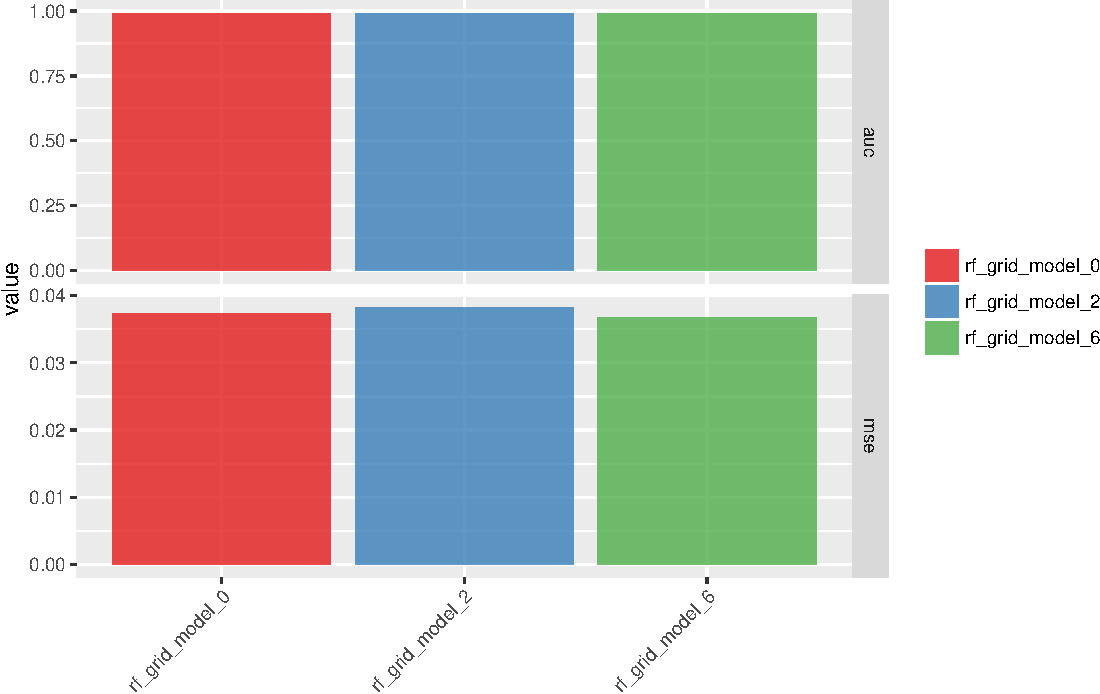
\includegraphics[width=1\textwidth]{webinar_code_files/figure-latex/auc_mse-1.pdf} \end{center}
\end{frame}

\note{
	In statistics, the mean squared error (MSE) or mean squared deviation (MSD) of an estimator (of a procedure for estimating an unobserved quantity) measures the average of the squares of the errors or deviations?that is, the difference between the estimator and what is estimated. MSE is a risk function, corresponding to the expected value of the squared error loss or quadratic loss. The difference occurs because of randomness or because the estimator doesn't account for information that could produce a more accurate estimate.[1]
	
	The MSE is a measure of the quality of an estimator?it is always non-negative, and values closer to zero are better.
	
	The MSE is the second moment (about the origin) of the error, and thus incorporates both the variance of the estimator and its bias. For an unbiased estimator, the MSE is the variance of the estimator. Like the variance, MSE has the same units of measurement as the square of the quantity being estimated. In an analogy to standard deviation, taking the square root of MSE yields the root-mean-square error or root-mean-square deviation (RMSE or RMSD), which has the same units as the quantity being estimated; for an unbiased estimator, the RMSE is the square root of the variance, known as the standard deviation.
	
	The MSE assesses the quality of an estimator (i.e., a mathematical function mapping a sample of data to a parameter of the population from which the data is sampled) or a predictor (i.e., a function mapping arbitrary inputs to a sample of values of some random variable). Definition of an MSE differs according to whether one is describing an estimator or a predictor.
}

\begin{frame}
	\frametitle{Predictions on test data}
	
	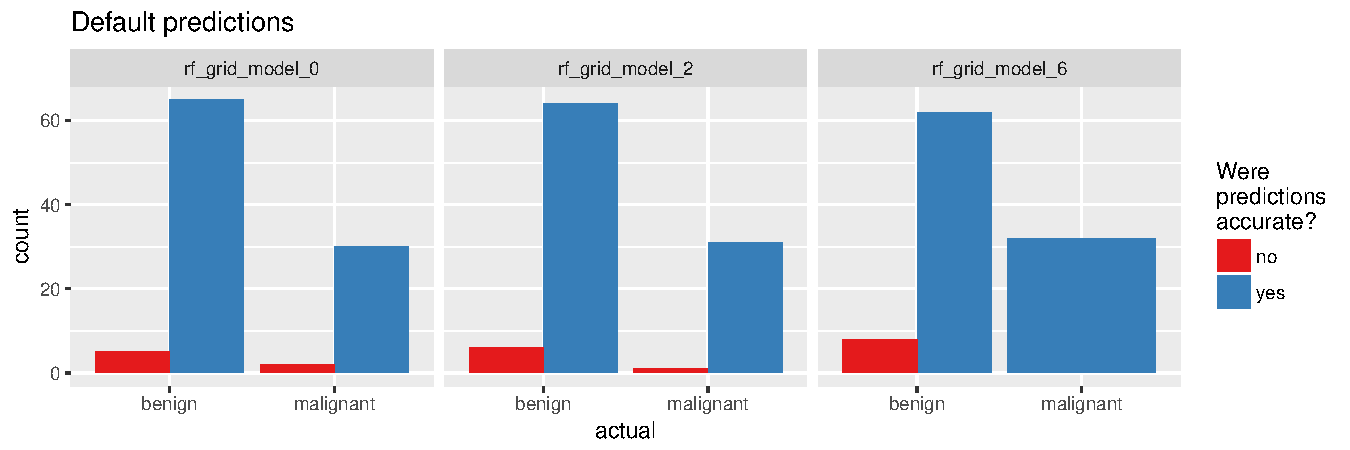
\includegraphics[width=1\textwidth]{webinar_code_files/figure-latex/final_predictions_rf-1.pdf} 

	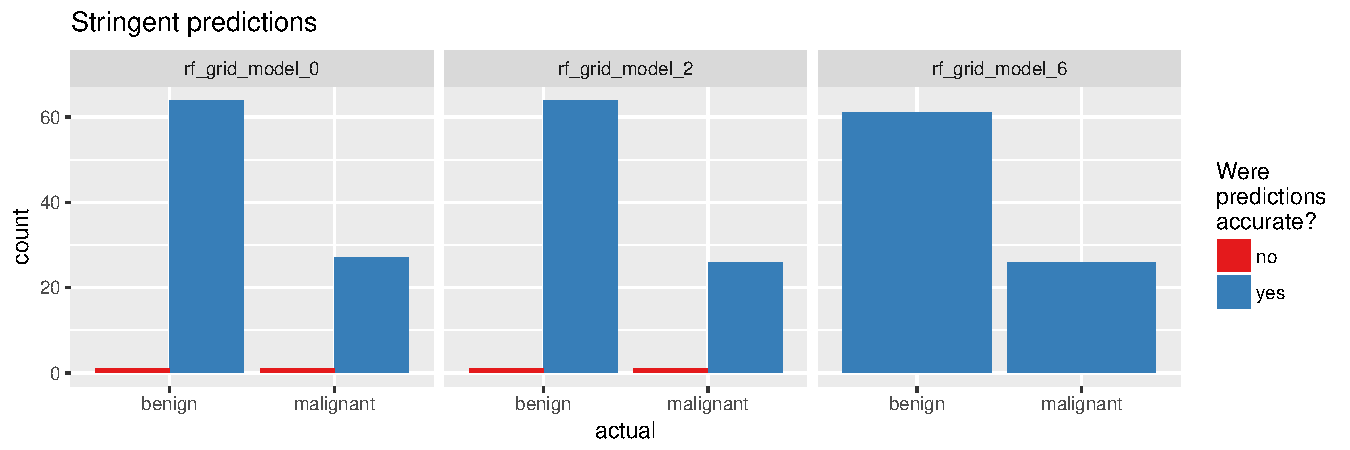
\includegraphics[width=1\textwidth]{webinar_code_files/figure-latex/final_predictions_rf-2.pdf} 
\end{frame}


% accuracy
% Kappa

\begin{frame}[plain, c]
	
	\begin{center}
		\usebeamerfont*{frametitle} \usebeamercolor[fg]{frametitle} {\Huge \textbf{Take home messages:}}
	\end{center}
	
	\vspace{0.5cm}
	
	\begin{itemize}
		\item ...
	\end{itemize}
\end{frame}

\begin{frame}
	\frametitle{Outlook}
	
	\begin{itemize}
		\item `big data' needs to be big!
		\item for really meaningful models, data needs to be shared
		\item the more data, the more accurate and generalizable the models will be
		\item issues: privacy, platform, quality standards
		\item ML could make health care more cost-effective by reducing the energy required for interpretation
	\end{itemize}
\end{frame}

%%%%%%%%%%%%%%%%%%%%%

\begin{frame}[plain, c]
	
	\begin{center}
	\usebeamerfont*{frametitle} \usebeamercolor[fg]{frametitle} {\Huge \textbf{Thank you for your attention!}}
	\end{center}

	\vspace{0.5cm}

	\begin{center}
		\usebeamerfont*{frametitle} {\huge Questions?}
	\end{center}

	\vspace{0.5cm}
	
	Slides and code will be available on Github: \href{https://github.com/ShirinG/Webinar_ML_for_disease}{https://github.com/ShirinG/Webinar\_ML\_for\_disease} \\
	
	\vspace{0.5cm}
	
	Code will also be on my website: \href{https://shiring.github.io}{https://shiring.github.io} \\
	
	\vspace{0.5cm}
	
	\href{mailto:shirin.glander@wwu.de}{shirin.glander@wwu.de} \\
	
\end{frame}

\end{document}